\documentclass[twoside]{book}

% Packages required by doxygen
\usepackage{fixltx2e}
\usepackage{calc}
\usepackage{doxygen}
\usepackage{graphicx}
\usepackage[utf8]{inputenc}
\usepackage{makeidx}
\usepackage{multicol}
\usepackage{multirow}
\PassOptionsToPackage{warn}{textcomp}
\usepackage{textcomp}
\usepackage[nointegrals]{wasysym}
\usepackage[table]{xcolor}

% Font selection
\usepackage[T1]{fontenc}
\usepackage{mathptmx}
\usepackage[scaled=.90]{helvet}
\usepackage{courier}
\usepackage{amssymb}
\usepackage{sectsty}
\renewcommand{\familydefault}{\sfdefault}
\allsectionsfont{%
  \fontseries{bc}\selectfont%
  \color{darkgray}%
}
\renewcommand{\DoxyLabelFont}{%
  \fontseries{bc}\selectfont%
  \color{darkgray}%
}
\newcommand{\+}{\discretionary{\mbox{\scriptsize$\hookleftarrow$}}{}{}}

% Page & text layout
\usepackage{geometry}
\geometry{%
  a4paper,%
  top=2.5cm,%
  bottom=2.5cm,%
  left=2.5cm,%
  right=2.5cm%
}
\tolerance=750
\hfuzz=15pt
\hbadness=750
\setlength{\emergencystretch}{15pt}
\setlength{\parindent}{0cm}
\setlength{\parskip}{0.2cm}
\makeatletter
\renewcommand{\paragraph}{%
  \@startsection{paragraph}{4}{0ex}{-1.0ex}{1.0ex}{%
    \normalfont\normalsize\bfseries\SS@parafont%
  }%
}
\renewcommand{\subparagraph}{%
  \@startsection{subparagraph}{5}{0ex}{-1.0ex}{1.0ex}{%
    \normalfont\normalsize\bfseries\SS@subparafont%
  }%
}
\makeatother

% Headers & footers
\usepackage{fancyhdr}
\pagestyle{fancyplain}
\fancyhead[LE]{\fancyplain{}{\bfseries\thepage}}
\fancyhead[CE]{\fancyplain{}{}}
\fancyhead[RE]{\fancyplain{}{\bfseries\leftmark}}
\fancyhead[LO]{\fancyplain{}{\bfseries\rightmark}}
\fancyhead[CO]{\fancyplain{}{}}
\fancyhead[RO]{\fancyplain{}{\bfseries\thepage}}
\fancyfoot[LE]{\fancyplain{}{}}
\fancyfoot[CE]{\fancyplain{}{}}
\fancyfoot[RE]{\fancyplain{}{\bfseries\scriptsize Generated on Tue Aug 11 2015 14\+:50\+:19 for Ace Engine by Doxygen }}
\fancyfoot[LO]{\fancyplain{}{\bfseries\scriptsize Generated on Tue Aug 11 2015 14\+:50\+:19 for Ace Engine by Doxygen }}
\fancyfoot[CO]{\fancyplain{}{}}
\fancyfoot[RO]{\fancyplain{}{}}
\renewcommand{\footrulewidth}{0.4pt}
\renewcommand{\chaptermark}[1]{%
  \markboth{#1}{}%
}
\renewcommand{\sectionmark}[1]{%
  \markright{\thesection\ #1}%
}

% Indices & bibliography
\usepackage{natbib}
\usepackage[titles]{tocloft}
\setcounter{tocdepth}{3}
\setcounter{secnumdepth}{5}
\makeindex

% Hyperlinks (required, but should be loaded last)
\usepackage{ifpdf}
\ifpdf
  \usepackage[pdftex,pagebackref=true]{hyperref}
\else
  \usepackage[ps2pdf,pagebackref=true]{hyperref}
\fi
\hypersetup{%
  colorlinks=true,%
  linkcolor=blue,%
  citecolor=blue,%
  unicode%
}

% Custom commands
\newcommand{\clearemptydoublepage}{%
  \newpage{\pagestyle{empty}\cleardoublepage}%
}


%===== C O N T E N T S =====

\begin{document}

% Titlepage & ToC
\hypersetup{pageanchor=false,
             bookmarks=true,
             bookmarksnumbered=true,
             pdfencoding=unicode
            }
\pagenumbering{roman}
\begin{titlepage}
\vspace*{7cm}
\begin{center}%
{\Large Ace Engine }\\
\vspace*{1cm}
{\large Generated by Doxygen 1.8.8}\\
\vspace*{0.5cm}
{\small Tue Aug 11 2015 14:50:19}\\
\end{center}
\end{titlepage}
\clearemptydoublepage
\tableofcontents
\clearemptydoublepage
\pagenumbering{arabic}
\hypersetup{pageanchor=true}

%--- Begin generated contents ---
\chapter{Hierarchical Index}
\section{Class Hierarchy}
This inheritance list is sorted roughly, but not completely, alphabetically\+:\begin{DoxyCompactList}
\item \contentsline{section}{Audio\+System}{\pageref{class_audio_system}}{}
\item \contentsline{section}{Camera\+Component}{\pageref{struct_camera_component}}{}
\item \contentsline{section}{Camera\+System}{\pageref{class_camera_system}}{}
\item \contentsline{section}{Capsule\+Collider\+Component}{\pageref{struct_capsule_collider_component}}{}
\item \contentsline{section}{Character\+Controller\+Component}{\pageref{struct_character_controller_component}}{}
\item \contentsline{section}{Component\+Serializer}{\pageref{class_component_serializer}}{}
\item \contentsline{section}{Component\+World$<$ T $>$}{\pageref{class_component_world}}{}
\item \contentsline{section}{Packed\+Array$<$ T $>$\+:\+:Const\+Iterator}{\pageref{class_packed_array_1_1_const_iterator}}{}
\item \contentsline{section}{Entity\+World}{\pageref{class_entity_world}}{}
\item \contentsline{section}{events\+:\+:Event\+Data}{\pageref{structevents_1_1_event_data}}{}
\begin{DoxyCompactList}
\item \contentsline{section}{events\+:\+:Mouse\+Moved\+Data}{\pageref{structevents_1_1_mouse_moved_data}}{}
\item \contentsline{section}{events\+:\+:Play\+Sound\+Data}{\pageref{structevents_1_1_play_sound_data}}{}
\item \contentsline{section}{events\+:\+:Window\+Created\+Data}{\pageref{structevents_1_1_window_created_data}}{}
\end{DoxyCompactList}
\item \contentsline{section}{events\+:\+:Event\+System}{\pageref{classevents_1_1_event_system}}{}
\item \contentsline{section}{Game}{\pageref{class_game}}{}
\item \contentsline{section}{Input\+System}{\pageref{class_input_system}}{}
\item \contentsline{section}{Packed\+Array$<$ T $>$\+:\+:Iterator}{\pageref{class_packed_array_1_1_iterator}}{}
\item \contentsline{section}{Light\+Component}{\pageref{struct_light_component}}{}
\item \contentsline{section}{Material}{\pageref{struct_material}}{}
\item \contentsline{section}{Mesh\+Component}{\pageref{struct_mesh_component}}{}
\item \contentsline{section}{Music\+Component}{\pageref{struct_music_component}}{}
\item \contentsline{section}{Packed\+Array$<$ T $>$}{\pageref{class_packed_array}}{}
\item \contentsline{section}{Physics\+System}{\pageref{class_physics_system}}{}
\item \contentsline{section}{Player\+Component}{\pageref{struct_player_component}}{}
\item \contentsline{section}{Render\+System}{\pageref{class_render_system}}{}
\item \contentsline{section}{Resource\+Loader$<$ T $>$}{\pageref{class_resource_loader}}{}
\item \contentsline{section}{Resource\+Loader$<$ Shader $>$}{\pageref{class_resource_loader}}{}
\item \contentsline{section}{Resource\+Loader$<$ Sound $>$}{\pageref{class_resource_loader}}{}
\item \contentsline{section}{Resource\+Loader$<$ Texture $>$}{\pageref{class_resource_loader}}{}
\item \contentsline{section}{Rigidbody\+Component}{\pageref{struct_rigidbody_component}}{}
\item \contentsline{section}{Scene\+Importer}{\pageref{class_scene_importer}}{}
\item \contentsline{section}{Scene\+Loader}{\pageref{class_scene_loader}}{}
\item \contentsline{section}{Shader}{\pageref{struct_shader}}{}
\item \contentsline{section}{Skybox\+Component}{\pageref{struct_skybox_component}}{}
\item \contentsline{section}{Sound}{\pageref{struct_sound}}{}
\item \contentsline{section}{Terrain\+Component}{\pageref{struct_terrain_component}}{}
\item \contentsline{section}{Terrain\+System}{\pageref{class_terrain_system}}{}
\item \contentsline{section}{Terrain\+Vertex\+Data}{\pageref{struct_terrain_vertex_data}}{}
\item \contentsline{section}{Texture}{\pageref{struct_texture}}{}
\item \contentsline{section}{Transform\+Component}{\pageref{struct_transform_component}}{}
\item \contentsline{section}{Vertex\+Data}{\pageref{struct_vertex_data}}{}
\end{DoxyCompactList}

\chapter{Class Index}
\section{Class List}
Here are the classes, structs, unions and interfaces with brief descriptions\+:\begin{DoxyCompactList}
\item\contentsline{section}{\hyperlink{class_audio_system}{Audio\+System} }{\pageref{class_audio_system}}{}
\item\contentsline{section}{\hyperlink{struct_camera_component}{Camera\+Component} }{\pageref{struct_camera_component}}{}
\item\contentsline{section}{\hyperlink{class_camera_system}{Camera\+System} }{\pageref{class_camera_system}}{}
\item\contentsline{section}{\hyperlink{struct_capsule_collider_component}{Capsule\+Collider\+Component} }{\pageref{struct_capsule_collider_component}}{}
\item\contentsline{section}{\hyperlink{struct_character_controller_component}{Character\+Controller\+Component} }{\pageref{struct_character_controller_component}}{}
\item\contentsline{section}{\hyperlink{class_component_serializer}{Component\+Serializer} }{\pageref{class_component_serializer}}{}
\item\contentsline{section}{\hyperlink{class_component_world}{Component\+World$<$ T $>$} }{\pageref{class_component_world}}{}
\item\contentsline{section}{\hyperlink{class_packed_array_1_1_const_iterator}{Packed\+Array$<$ T $>$\+::\+Const\+Iterator} }{\pageref{class_packed_array_1_1_const_iterator}}{}
\item\contentsline{section}{\hyperlink{class_entity_world}{Entity\+World} }{\pageref{class_entity_world}}{}
\item\contentsline{section}{\hyperlink{structevents_1_1_event_data}{events\+::\+Event\+Data} }{\pageref{structevents_1_1_event_data}}{}
\item\contentsline{section}{\hyperlink{classevents_1_1_event_system}{events\+::\+Event\+System} }{\pageref{classevents_1_1_event_system}}{}
\item\contentsline{section}{\hyperlink{class_game}{Game} }{\pageref{class_game}}{}
\item\contentsline{section}{\hyperlink{class_input_system}{Input\+System} }{\pageref{class_input_system}}{}
\item\contentsline{section}{\hyperlink{class_packed_array_1_1_iterator}{Packed\+Array$<$ T $>$\+::\+Iterator} }{\pageref{class_packed_array_1_1_iterator}}{}
\item\contentsline{section}{\hyperlink{struct_light_component}{Light\+Component} }{\pageref{struct_light_component}}{}
\item\contentsline{section}{\hyperlink{struct_material}{Material} }{\pageref{struct_material}}{}
\item\contentsline{section}{\hyperlink{struct_mesh_component}{Mesh\+Component} }{\pageref{struct_mesh_component}}{}
\item\contentsline{section}{\hyperlink{structevents_1_1_mouse_moved_data}{events\+::\+Mouse\+Moved\+Data} }{\pageref{structevents_1_1_mouse_moved_data}}{}
\item\contentsline{section}{\hyperlink{struct_music_component}{Music\+Component} }{\pageref{struct_music_component}}{}
\item\contentsline{section}{\hyperlink{class_packed_array}{Packed\+Array$<$ T $>$} }{\pageref{class_packed_array}}{}
\item\contentsline{section}{\hyperlink{class_physics_system}{Physics\+System} }{\pageref{class_physics_system}}{}
\item\contentsline{section}{\hyperlink{struct_player_component}{Player\+Component} }{\pageref{struct_player_component}}{}
\item\contentsline{section}{\hyperlink{structevents_1_1_play_sound_data}{events\+::\+Play\+Sound\+Data} }{\pageref{structevents_1_1_play_sound_data}}{}
\item\contentsline{section}{\hyperlink{class_render_system}{Render\+System} }{\pageref{class_render_system}}{}
\item\contentsline{section}{\hyperlink{class_resource_loader}{Resource\+Loader$<$ T $>$} }{\pageref{class_resource_loader}}{}
\item\contentsline{section}{\hyperlink{struct_rigidbody_component}{Rigidbody\+Component} }{\pageref{struct_rigidbody_component}}{}
\item\contentsline{section}{\hyperlink{class_scene_importer}{Scene\+Importer} }{\pageref{class_scene_importer}}{}
\item\contentsline{section}{\hyperlink{class_scene_loader}{Scene\+Loader} }{\pageref{class_scene_loader}}{}
\item\contentsline{section}{\hyperlink{struct_shader}{Shader} }{\pageref{struct_shader}}{}
\item\contentsline{section}{\hyperlink{struct_skybox_component}{Skybox\+Component} }{\pageref{struct_skybox_component}}{}
\item\contentsline{section}{\hyperlink{struct_sound}{Sound} }{\pageref{struct_sound}}{}
\item\contentsline{section}{\hyperlink{struct_terrain_component}{Terrain\+Component} }{\pageref{struct_terrain_component}}{}
\item\contentsline{section}{\hyperlink{class_terrain_system}{Terrain\+System} }{\pageref{class_terrain_system}}{}
\item\contentsline{section}{\hyperlink{struct_terrain_vertex_data}{Terrain\+Vertex\+Data} }{\pageref{struct_terrain_vertex_data}}{}
\item\contentsline{section}{\hyperlink{struct_texture}{Texture} }{\pageref{struct_texture}}{}
\item\contentsline{section}{\hyperlink{struct_transform_component}{Transform\+Component} }{\pageref{struct_transform_component}}{}
\item\contentsline{section}{\hyperlink{struct_vertex_data}{Vertex\+Data} }{\pageref{struct_vertex_data}}{}
\item\contentsline{section}{\hyperlink{structevents_1_1_window_created_data}{events\+::\+Window\+Created\+Data} }{\pageref{structevents_1_1_window_created_data}}{}
\end{DoxyCompactList}

\chapter{Class Documentation}
\hypertarget{class_audio_system}{}\section{Audio\+System Class Reference}
\label{class_audio_system}\index{Audio\+System@{Audio\+System}}
\subsection*{Public Member Functions}
\begin{DoxyCompactItemize}
\item 
\hypertarget{class_audio_system_accf9fda76c14df05603132421c43b7e4}{}{\bfseries Audio\+System} (\hyperlink{class_entity_world}{Entity\+World} $\ast$entity\+World)\label{class_audio_system_accf9fda76c14df05603132421c43b7e4}

\item 
\hypertarget{class_audio_system_a4edf9ab7c54d773292e712a353d0b406}{}void {\bfseries start} ()\label{class_audio_system_a4edf9ab7c54d773292e712a353d0b406}

\item 
\hypertarget{class_audio_system_a1e3849471338bf0bf38fbc96357dc16f}{}void {\bfseries update} (float delta\+Time)\label{class_audio_system_a1e3849471338bf0bf38fbc96357dc16f}

\end{DoxyCompactItemize}


The documentation for this class was generated from the following files\+:\begin{DoxyCompactItemize}
\item 
C\+:/\+Users/\+Simon/\+Documents/\+Visual Studio 2013/\+Projects/\+Ace\+Engine/\+Source/\+Ace\+Engine/Audio\+System.\+h\item 
C\+:/\+Users/\+Simon/\+Documents/\+Visual Studio 2013/\+Projects/\+Ace\+Engine/\+Source/\+Ace\+Engine/Audio\+System.\+cpp\end{DoxyCompactItemize}

\hypertarget{struct_camera_component}{}\section{Camera\+Component Struct Reference}
\label{struct_camera_component}\index{Camera\+Component@{Camera\+Component}}
\subsection*{Public Attributes}
\begin{DoxyCompactItemize}
\item 
\hypertarget{struct_camera_component_a6cabfd0a26360caba0f38a23c0bce354}{}Entity\+Id {\bfseries entity\+Id}\label{struct_camera_component_a6cabfd0a26360caba0f38a23c0bce354}

\item 
\hypertarget{struct_camera_component_a9de6948b7499d6d214842b69e1f95855}{}Element\+Id {\bfseries component\+Id}\label{struct_camera_component_a9de6948b7499d6d214842b69e1f95855}

\item 
\hypertarget{struct_camera_component_ae106ba028a02a4f99b19f9ca10af17ce}{}glm\+::vec3 {\bfseries direction} = glm\+::vec3(0.\+0f, 0.\+0f, 1.\+0f)\label{struct_camera_component_ae106ba028a02a4f99b19f9ca10af17ce}

\item 
\hypertarget{struct_camera_component_a9ec51727d0c75fc7ee9aefbf790a83d1}{}glm\+::vec3 {\bfseries forward} = glm\+::vec3(0.\+0f, 0.\+0f, 1.\+0f)\label{struct_camera_component_a9ec51727d0c75fc7ee9aefbf790a83d1}

\item 
\hypertarget{struct_camera_component_a62040ca115beaa48627fe56d330647c0}{}glm\+::vec3 {\bfseries right} = glm\+::vec3(1.\+0f, 0.\+0f, 0.\+0f)\label{struct_camera_component_a62040ca115beaa48627fe56d330647c0}

\item 
\hypertarget{struct_camera_component_a639f14e0057198d84ed8de71c3df3303}{}glm\+::vec3 {\bfseries up} = glm\+::vec3(0.\+0, 1.\+0f, 0.\+0f)\label{struct_camera_component_a639f14e0057198d84ed8de71c3df3303}

\item 
\hypertarget{struct_camera_component_acac8dfce611858ae1b3df9fc5233fe6b}{}glm\+::vec2 {\bfseries viewport\+Size}\label{struct_camera_component_acac8dfce611858ae1b3df9fc5233fe6b}

\item 
\hypertarget{struct_camera_component_ab56cb75b0f826bd88f30fdcd359f1439}{}float {\bfseries pitch} = 0.\+0f\label{struct_camera_component_ab56cb75b0f826bd88f30fdcd359f1439}

\item 
\hypertarget{struct_camera_component_a5c4e3536d3e7f15313f1a2b83a2095d9}{}float {\bfseries yaw} = 0.\+0f\label{struct_camera_component_a5c4e3536d3e7f15313f1a2b83a2095d9}

\item 
\hypertarget{struct_camera_component_aaa1e1e7bf6661a77d556306367bbcc41}{}float {\bfseries roll} = 0.\+0f\label{struct_camera_component_aaa1e1e7bf6661a77d556306367bbcc41}

\item 
\hypertarget{struct_camera_component_ad191cef2c4cd0c9fff185bf41fbebb88}{}float {\bfseries fov} = 65.\+0f\label{struct_camera_component_ad191cef2c4cd0c9fff185bf41fbebb88}

\item 
\hypertarget{struct_camera_component_a44ff1ccd1b703e9ead065969be8fb044}{}float {\bfseries z\+Near} = 0.\+1f\label{struct_camera_component_a44ff1ccd1b703e9ead065969be8fb044}

\item 
\hypertarget{struct_camera_component_aea7d06f025c69f1db065e04bd477f19c}{}float {\bfseries z\+Far} = 1000.\+0f\label{struct_camera_component_aea7d06f025c69f1db065e04bd477f19c}

\end{DoxyCompactItemize}


The documentation for this struct was generated from the following file\+:\begin{DoxyCompactItemize}
\item 
C\+:/\+Users/\+Simon/\+Documents/\+Visual Studio 2013/\+Projects/\+Ace\+Engine/\+Source/\+Ace\+Engine/Camera\+Component.\+h\end{DoxyCompactItemize}

\hypertarget{class_camera_system}{}\section{Camera\+System Class Reference}
\label{class_camera_system}\index{Camera\+System@{Camera\+System}}
\subsection*{Public Member Functions}
\begin{DoxyCompactItemize}
\item 
\hypertarget{class_camera_system_aa014df0181c358c23db31610643efb07}{}{\bfseries Camera\+System} (\hyperlink{class_entity_world}{Entity\+World} $\ast$entity\+World)\label{class_camera_system_aa014df0181c358c23db31610643efb07}

\item 
\hypertarget{class_camera_system_a39564045e7ef0ef7171f82e55586e4c9}{}void {\bfseries start} ()\label{class_camera_system_a39564045e7ef0ef7171f82e55586e4c9}

\item 
\hypertarget{class_camera_system_a09f1bfd9b78bba8e7f30c36ad8a65cdd}{}void {\bfseries update} (float delta\+Time)\label{class_camera_system_a09f1bfd9b78bba8e7f30c36ad8a65cdd}

\end{DoxyCompactItemize}


The documentation for this class was generated from the following files\+:\begin{DoxyCompactItemize}
\item 
C\+:/\+Users/\+Simon/\+Documents/\+Visual Studio 2013/\+Projects/\+Ace\+Engine/\+Source/\+Ace\+Engine/Camera\+System.\+h\item 
C\+:/\+Users/\+Simon/\+Documents/\+Visual Studio 2013/\+Projects/\+Ace\+Engine/\+Source/\+Ace\+Engine/Camera\+System.\+cpp\end{DoxyCompactItemize}

\hypertarget{struct_capsule_collider_component}{}\section{Capsule\+Collider\+Component Struct Reference}
\label{struct_capsule_collider_component}\index{Capsule\+Collider\+Component@{Capsule\+Collider\+Component}}
\subsection*{Public Attributes}
\begin{DoxyCompactItemize}
\item 
\hypertarget{struct_capsule_collider_component_a756eb9730241eb966a9edf015ac82ed4}{}Entity\+Id {\bfseries entity\+Id}\label{struct_capsule_collider_component_a756eb9730241eb966a9edf015ac82ed4}

\item 
\hypertarget{struct_capsule_collider_component_abe06586e7c28b7de581dd86855dc3761}{}Element\+Id {\bfseries component\+Id}\label{struct_capsule_collider_component_abe06586e7c28b7de581dd86855dc3761}

\item 
\hypertarget{struct_capsule_collider_component_a18d189734f90108412ea264128a09d1d}{}physx\+::\+Px\+Rigid\+Static $\ast$ {\bfseries static\+Body} = nullptr\label{struct_capsule_collider_component_a18d189734f90108412ea264128a09d1d}

\item 
\hypertarget{struct_capsule_collider_component_a1be770ca35c7d99ef4999279da9fe082}{}physx\+::\+Px\+Shape $\ast$ {\bfseries shape} = nullptr\label{struct_capsule_collider_component_a1be770ca35c7d99ef4999279da9fe082}

\item 
\hypertarget{struct_capsule_collider_component_a552a76c9b7712d1c1032a21e6a5fbeed}{}physx\+::\+Px\+Material $\ast$ {\bfseries material} = nullptr\label{struct_capsule_collider_component_a552a76c9b7712d1c1032a21e6a5fbeed}

\item 
\hypertarget{struct_capsule_collider_component_ae89b8784348c24165911a2d199049f0e}{}float {\bfseries radius} = 0.\+5f\label{struct_capsule_collider_component_ae89b8784348c24165911a2d199049f0e}

\item 
\hypertarget{struct_capsule_collider_component_a21126952a21245d697d042c741901eca}{}float {\bfseries height} = 1.\+0f\label{struct_capsule_collider_component_a21126952a21245d697d042c741901eca}

\item 
\hypertarget{struct_capsule_collider_component_a83dfd7b15c450998654ed85b5705e45d}{}bool {\bfseries is\+Dynamic} = false\label{struct_capsule_collider_component_a83dfd7b15c450998654ed85b5705e45d}

\end{DoxyCompactItemize}


The documentation for this struct was generated from the following file\+:\begin{DoxyCompactItemize}
\item 
C\+:/\+Users/\+Simon/\+Documents/\+Visual Studio 2013/\+Projects/\+Ace\+Engine/\+Source/\+Ace\+Engine/Capsule\+Collider\+Component.\+h\end{DoxyCompactItemize}

\hypertarget{struct_character_controller_component}{}\section{Character\+Controller\+Component Struct Reference}
\label{struct_character_controller_component}\index{Character\+Controller\+Component@{Character\+Controller\+Component}}
\subsection*{Public Attributes}
\begin{DoxyCompactItemize}
\item 
\hypertarget{struct_character_controller_component_ad5abc3869c313e3df7da87ed85b71867}{}glm\+::vec3 {\bfseries force} = glm\+::vec3(0.\+0f)\label{struct_character_controller_component_ad5abc3869c313e3df7da87ed85b71867}

\item 
\hypertarget{struct_character_controller_component_ab9f6e5b90ab313017bb82c4bae1c1078}{}glm\+::vec3 {\bfseries velocity} = glm\+::vec3(0.\+0f)\label{struct_character_controller_component_ab9f6e5b90ab313017bb82c4bae1c1078}

\item 
\hypertarget{struct_character_controller_component_a0385a62a149f136631dc3e48e6771a00}{}Entity\+Id {\bfseries entity\+Id}\label{struct_character_controller_component_a0385a62a149f136631dc3e48e6771a00}

\item 
\hypertarget{struct_character_controller_component_a43b7513a8d1c35d9f33d74bd3a405b87}{}Element\+Id {\bfseries component\+Id}\label{struct_character_controller_component_a43b7513a8d1c35d9f33d74bd3a405b87}

\item 
\hypertarget{struct_character_controller_component_a86a1379146c10658930d3276f0aa31b5}{}physx\+::\+Px\+Controller $\ast$ {\bfseries controller} = nullptr\label{struct_character_controller_component_a86a1379146c10658930d3276f0aa31b5}

\item 
\hypertarget{struct_character_controller_component_ae5032631093c4e7c5ea51b52e701ee32}{}float {\bfseries radius} = 0.\+5f\label{struct_character_controller_component_ae5032631093c4e7c5ea51b52e701ee32}

\item 
\hypertarget{struct_character_controller_component_a608901a7230c233baa8c88b3b42cdc32}{}float {\bfseries height} = 1.\+8f\label{struct_character_controller_component_a608901a7230c233baa8c88b3b42cdc32}

\item 
\hypertarget{struct_character_controller_component_aba50ef8c828907c8f9c1043eca6ad326}{}float {\bfseries slope\+Limit} = 0.\+5f\label{struct_character_controller_component_aba50ef8c828907c8f9c1043eca6ad326}

\item 
\hypertarget{struct_character_controller_component_a032257274fe5c5e10e5fec5627e62c3e}{}bool {\bfseries is\+On\+Ground} = false\label{struct_character_controller_component_a032257274fe5c5e10e5fec5627e62c3e}

\end{DoxyCompactItemize}


The documentation for this struct was generated from the following file\+:\begin{DoxyCompactItemize}
\item 
C\+:/\+Users/\+Simon/\+Documents/\+Visual Studio 2013/\+Projects/\+Ace\+Engine/\+Source/\+Ace\+Engine/Character\+Controller\+Component.\+h\end{DoxyCompactItemize}

\hypertarget{class_component_serializer}{}\section{Component\+Serializer Class Reference}
\label{class_component_serializer}\index{Component\+Serializer@{Component\+Serializer}}
\subsection*{Public Member Functions}
\begin{DoxyCompactItemize}
\item 
\hypertarget{class_component_serializer_ab5fd892a3aef23f30339b3eda3494f31}{}{\bfseries Component\+Serializer} (\hyperlink{class_entity_world}{Entity\+World} $\ast$entity\+World, \hyperlink{class_resource_loader}{Resource\+Loader}$<$ \hyperlink{struct_texture}{Texture} $>$ $\ast$texture\+Loader, \hyperlink{class_resource_loader}{Resource\+Loader}$<$ \hyperlink{struct_shader}{Shader} $>$ $\ast$shader\+Loader)\label{class_component_serializer_ab5fd892a3aef23f30339b3eda3494f31}

\item 
\hypertarget{class_component_serializer_ab0bfc10077164ec952d42ffd91c85807}{}void {\bfseries deserialize} (const std\+::string type\+Name, std\+::unordered\+\_\+map$<$ std\+::string, std\+::string $>$ \&members)\label{class_component_serializer_ab0bfc10077164ec952d42ffd91c85807}

\end{DoxyCompactItemize}


The documentation for this class was generated from the following files\+:\begin{DoxyCompactItemize}
\item 
C\+:/\+Users/\+Simon/\+Documents/\+Visual Studio 2013/\+Projects/\+Ace\+Engine/\+Source/\+Ace\+Engine/Component\+Serializer.\+h\item 
C\+:/\+Users/\+Simon/\+Documents/\+Visual Studio 2013/\+Projects/\+Ace\+Engine/\+Source/\+Ace\+Engine/Component\+Serializer.\+cpp\end{DoxyCompactItemize}

\hypertarget{class_component_world}{}\section{Component\+World$<$ T $>$ Class Template Reference}
\label{class_component_world}\index{Component\+World$<$ T $>$@{Component\+World$<$ T $>$}}
\subsection*{Public Member Functions}
\begin{DoxyCompactItemize}
\item 
\hypertarget{class_component_world_a156ba0ac393da228f164287ce911fffc}{}{\bfseries Component\+World} (size\+\_\+t element\+Count)\label{class_component_world_a156ba0ac393da228f164287ce911fffc}

\item 
\hypertarget{class_component_world_a75233dcb97d315d4e06a0f767b70f3a1}{}\hyperlink{class_packed_array}{Packed\+Array}$<$ T $>$ \& {\bfseries get\+Array} ()\label{class_component_world_a75233dcb97d315d4e06a0f767b70f3a1}

\item 
\hypertarget{class_component_world_a50bb6dc0183362e0748a66abbe21410e}{}T $\ast$ {\bfseries get} (Element\+Id component\+Id)\label{class_component_world_a50bb6dc0183362e0748a66abbe21410e}

\item 
\hypertarget{class_component_world_a02a565a807f1625be89091f15e906105}{}T $\ast$ {\bfseries get\+First} (Entity\+Id id)\label{class_component_world_a02a565a807f1625be89091f15e906105}

\item 
\hypertarget{class_component_world_aba738be57cef4cf6c6791019f3a318a7}{}T $\ast$ {\bfseries add} (Entity\+Id id)\label{class_component_world_aba738be57cef4cf6c6791019f3a318a7}

\item 
\hypertarget{class_component_world_aa3b8a211c00d83f93e20780f036b8260}{}void {\bfseries remove} (Entity\+Id entity\+Id, Element\+Id component\+Id)\label{class_component_world_aa3b8a211c00d83f93e20780f036b8260}

\item 
\hypertarget{class_component_world_ae8a8cb1587089ff2454cdcb010fc3d8d}{}bool {\bfseries exist} (Entity\+Id id)\label{class_component_world_ae8a8cb1587089ff2454cdcb010fc3d8d}

\end{DoxyCompactItemize}


The documentation for this class was generated from the following file\+:\begin{DoxyCompactItemize}
\item 
C\+:/\+Users/\+Simon/\+Documents/\+Visual Studio 2013/\+Projects/\+Ace\+Engine/\+Source/\+Ace\+Engine/Component\+World.\+h\end{DoxyCompactItemize}

\hypertarget{class_packed_array_1_1_const_iterator}{}\section{Packed\+Array$<$ T $>$\+:\+:Const\+Iterator Class Reference}
\label{class_packed_array_1_1_const_iterator}\index{Packed\+Array$<$ T $>$\+::\+Const\+Iterator@{Packed\+Array$<$ T $>$\+::\+Const\+Iterator}}
\subsection*{Public Member Functions}
\begin{DoxyCompactItemize}
\item 
\hypertarget{class_packed_array_1_1_const_iterator_aaeaf61f1bafc89f343f00165e7c347e8}{}{\bfseries Const\+Iterator} (const \hyperlink{class_packed_array}{Packed\+Array}$<$ T $>$ $\ast$array, int index)\label{class_packed_array_1_1_const_iterator_aaeaf61f1bafc89f343f00165e7c347e8}

\item 
\hypertarget{class_packed_array_1_1_const_iterator_ab32cda8a1bbe7bb5b9b0e07e63751bf3}{}bool {\bfseries operator!=} (const \hyperlink{class_packed_array_1_1_const_iterator}{Const\+Iterator} \&other) const \label{class_packed_array_1_1_const_iterator_ab32cda8a1bbe7bb5b9b0e07e63751bf3}

\item 
\hypertarget{class_packed_array_1_1_const_iterator_af5d673ef73fab9a41d81c113517428db}{}T \& {\bfseries operator$\ast$} () const \label{class_packed_array_1_1_const_iterator_af5d673ef73fab9a41d81c113517428db}

\item 
\hypertarget{class_packed_array_1_1_const_iterator_abab1d92f9d0c129e1d9d7b91ced13f3b}{}const \hyperlink{class_packed_array_1_1_const_iterator}{Const\+Iterator} \& {\bfseries operator++} ()\label{class_packed_array_1_1_const_iterator_abab1d92f9d0c129e1d9d7b91ced13f3b}

\end{DoxyCompactItemize}


The documentation for this class was generated from the following file\+:\begin{DoxyCompactItemize}
\item 
C\+:/\+Users/\+Simon/\+Documents/\+Visual Studio 2013/\+Projects/\+Ace\+Engine/\+Source/\+Ace\+Engine/Packed\+Array.\+h\end{DoxyCompactItemize}

\hypertarget{class_entity_world}{}\section{Entity\+World Class Reference}
\label{class_entity_world}\index{Entity\+World@{Entity\+World}}
\subsection*{Public Member Functions}
\begin{DoxyCompactItemize}
\item 
\hypertarget{class_entity_world_ad0d89c5df1c32e4493ed1da216c97362}{}Entity\+Id {\bfseries get\+Unused\+Entity\+Id} ()\label{class_entity_world_ad0d89c5df1c32e4493ed1da216c97362}

\end{DoxyCompactItemize}


The documentation for this class was generated from the following files\+:\begin{DoxyCompactItemize}
\item 
C\+:/\+Users/\+Simon/\+Documents/\+Visual Studio 2013/\+Projects/\+Ace\+Engine/\+Source/\+Ace\+Engine/Entity\+World.\+h\item 
C\+:/\+Users/\+Simon/\+Documents/\+Visual Studio 2013/\+Projects/\+Ace\+Engine/\+Source/\+Ace\+Engine/Entity\+World.\+cpp\end{DoxyCompactItemize}

\hypertarget{structevents_1_1_event_data}{}\section{events\+:\+:Event\+Data Struct Reference}
\label{structevents_1_1_event_data}\index{events\+::\+Event\+Data@{events\+::\+Event\+Data}}
Inheritance diagram for events\+:\+:Event\+Data\+:\begin{figure}[H]
\begin{center}
\leavevmode
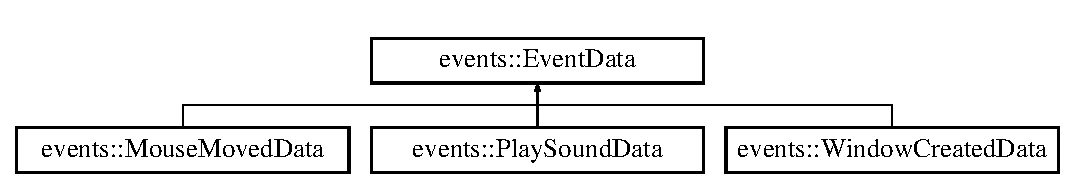
\includegraphics[height=2.000000cm]{structevents_1_1_event_data}
\end{center}
\end{figure}


The documentation for this struct was generated from the following file\+:\begin{DoxyCompactItemize}
\item 
C\+:/\+Users/\+Simon/\+Documents/\+Visual Studio 2013/\+Projects/\+Ace\+Engine/\+Source/\+Ace\+Engine/Event\+Data.\+h\end{DoxyCompactItemize}

\hypertarget{classevents_1_1_event_system}{}\section{events\+:\+:Event\+System Class Reference}
\label{classevents_1_1_event_system}\index{events\+::\+Event\+System@{events\+::\+Event\+System}}
\subsection*{Static Public Member Functions}
\begin{DoxyCompactItemize}
\item 
\hypertarget{classevents_1_1_event_system_a52182b9369c6211b65da6424e21ebe00}{}static void {\bfseries fire\+Event} (Event\+Type type, \hyperlink{structevents_1_1_event_data}{Event\+Data} $\ast$data)\label{classevents_1_1_event_system_a52182b9369c6211b65da6424e21ebe00}

\item 
\hypertarget{classevents_1_1_event_system_a7a76601b3d72825ddc1496c8ecfc466b}{}static void {\bfseries register\+Listener} (Event\+Type type, std\+::function$<$ void(\hyperlink{structevents_1_1_event_data}{Event\+Data} $\ast$)$>$ callback)\label{classevents_1_1_event_system_a7a76601b3d72825ddc1496c8ecfc466b}

\item 
\hypertarget{classevents_1_1_event_system_ab9b3f483b7eae6de6b3daa076290544b}{}static void {\bfseries remove\+Listener} (Event\+Type type)\label{classevents_1_1_event_system_ab9b3f483b7eae6de6b3daa076290544b}

\end{DoxyCompactItemize}


The documentation for this class was generated from the following files\+:\begin{DoxyCompactItemize}
\item 
C\+:/\+Users/\+Simon/\+Documents/\+Visual Studio 2013/\+Projects/\+Ace\+Engine/\+Source/\+Ace\+Engine/Event\+System.\+h\item 
C\+:/\+Users/\+Simon/\+Documents/\+Visual Studio 2013/\+Projects/\+Ace\+Engine/\+Source/\+Ace\+Engine/Event\+System.\+cpp\end{DoxyCompactItemize}

\hypertarget{class_game}{}\section{Game Class Reference}
\label{class_game}\index{Game@{Game}}
\subsection*{Public Member Functions}
\begin{DoxyCompactItemize}
\item 
\hypertarget{class_game_a3d9b98f7c4a96ecf578f75b96c9f0e90}{}void {\bfseries start} ()\label{class_game_a3d9b98f7c4a96ecf578f75b96c9f0e90}

\item 
\hypertarget{class_game_a1ab78f5ed0d5ea879157357cf2fb2afa}{}void {\bfseries run} ()\label{class_game_a1ab78f5ed0d5ea879157357cf2fb2afa}

\item 
\hypertarget{class_game_a17fbb36fd4a2085f9ff4f1fa93d7d08b}{}void {\bfseries stop} ()\label{class_game_a17fbb36fd4a2085f9ff4f1fa93d7d08b}

\end{DoxyCompactItemize}


The documentation for this class was generated from the following files\+:\begin{DoxyCompactItemize}
\item 
C\+:/\+Users/\+Simon/\+Documents/\+Visual Studio 2013/\+Projects/\+Ace\+Engine/\+Source/\+Ace\+Engine/Game.\+h\item 
C\+:/\+Users/\+Simon/\+Documents/\+Visual Studio 2013/\+Projects/\+Ace\+Engine/\+Source/\+Ace\+Engine/Game.\+cpp\end{DoxyCompactItemize}

\hypertarget{class_input_system}{}\section{Input\+System Class Reference}
\label{class_input_system}\index{Input\+System@{Input\+System}}
\subsection*{Public Types}
\begin{DoxyCompactItemize}
\item 
enum \hyperlink{class_input_system_ad2fd19ae265c6309c2f91259b757e8b4}{Key} \+: char \{ \\*
\hyperlink{class_input_system_ad2fd19ae265c6309c2f91259b757e8b4a88183b946cc5f0e8c96b2e66e1c74a7e}{Key\+::\+Unknown} = -\/1, 
\hyperlink{class_input_system_ad2fd19ae265c6309c2f91259b757e8b4a7fc56270e7a70fa81a5935b72eacbe29}{Key\+::\+A} = 0, 
\hyperlink{class_input_system_ad2fd19ae265c6309c2f91259b757e8b4a9d5ed678fe57bcca610140957afab571}{Key\+::\+B}, 
\hyperlink{class_input_system_ad2fd19ae265c6309c2f91259b757e8b4a0d61f8370cad1d412f80b84d143e1257}{Key\+::\+C}, 
\\*
\hyperlink{class_input_system_ad2fd19ae265c6309c2f91259b757e8b4af623e75af30e62bbd73d6df5b50bb7b5}{Key\+::\+D}, 
\hyperlink{class_input_system_ad2fd19ae265c6309c2f91259b757e8b4a3a3ea00cfc35332cedf6e5e9a32e94da}{Key\+::\+E}, 
\hyperlink{class_input_system_ad2fd19ae265c6309c2f91259b757e8b4a800618943025315f869e4e1f09471012}{Key\+::\+F}, 
\hyperlink{class_input_system_ad2fd19ae265c6309c2f91259b757e8b4adfcf28d0734569a6a693bc8194de62bf}{Key\+::\+G}, 
\\*
\hyperlink{class_input_system_ad2fd19ae265c6309c2f91259b757e8b4ac1d9f50f86825a1a2302ec2449c17196}{Key\+::\+H}, 
\hyperlink{class_input_system_ad2fd19ae265c6309c2f91259b757e8b4add7536794b63bf90eccfd37f9b147d7f}{Key\+::\+I}, 
\hyperlink{class_input_system_ad2fd19ae265c6309c2f91259b757e8b4aff44570aca8241914870afbc310cdb85}{Key\+::\+J}, 
\hyperlink{class_input_system_ad2fd19ae265c6309c2f91259b757e8b4aa5f3c6a11b03839d46af9fb43c97c188}{Key\+::\+K}, 
\\*
\hyperlink{class_input_system_ad2fd19ae265c6309c2f91259b757e8b4ad20caec3b48a1eef164cb4ca81ba2587}{Key\+::\+L}, 
\hyperlink{class_input_system_ad2fd19ae265c6309c2f91259b757e8b4a69691c7bdcc3ce6d5d8a1361f22d04ac}{Key\+::\+M}, 
\hyperlink{class_input_system_ad2fd19ae265c6309c2f91259b757e8b4a8d9c307cb7f3c4a32822a51922d1ceaa}{Key\+::\+N}, 
\hyperlink{class_input_system_ad2fd19ae265c6309c2f91259b757e8b4af186217753c37b9b9f958d906208506e}{Key\+::\+O}, 
\\*
\hyperlink{class_input_system_ad2fd19ae265c6309c2f91259b757e8b4a44c29edb103a2872f519ad0c9a0fdaaa}{Key\+::\+P}, 
\hyperlink{class_input_system_ad2fd19ae265c6309c2f91259b757e8b4af09564c9ca56850d4cd6b3319e541aee}{Key\+::\+Q}, 
\hyperlink{class_input_system_ad2fd19ae265c6309c2f91259b757e8b4ae1e1d3d40573127e9ee0480caf1283d6}{Key\+::\+R}, 
\hyperlink{class_input_system_ad2fd19ae265c6309c2f91259b757e8b4a5dbc98dcc983a70728bd082d1a47546e}{Key\+::\+S}, 
\\*
\hyperlink{class_input_system_ad2fd19ae265c6309c2f91259b757e8b4ab9ece18c950afbfa6b0fdbfa4ff731d3}{Key\+::\+T}, 
\hyperlink{class_input_system_ad2fd19ae265c6309c2f91259b757e8b4a4c614360da93c0a041b22e537de151eb}{Key\+::\+U}, 
\hyperlink{class_input_system_ad2fd19ae265c6309c2f91259b757e8b4a5206560a306a2e085a437fd258eb57ce}{Key\+::\+V}, 
\hyperlink{class_input_system_ad2fd19ae265c6309c2f91259b757e8b4a61e9c06ea9a85a5088a499df6458d276}{Key\+::\+W}, 
\\*
\hyperlink{class_input_system_ad2fd19ae265c6309c2f91259b757e8b4a02129bb861061d1a052c592e2dc6b383}{Key\+::\+X}, 
\hyperlink{class_input_system_ad2fd19ae265c6309c2f91259b757e8b4a57cec4137b614c87cb4e24a3d003a3e0}{Key\+::\+Y}, 
\hyperlink{class_input_system_ad2fd19ae265c6309c2f91259b757e8b4a21c2e59531c8710156d34a3c30ac81d5}{Key\+::\+Z}, 
\hyperlink{class_input_system_ad2fd19ae265c6309c2f91259b757e8b4a845787798a45b48e825e9b99a338537a}{Key\+::\+Num0}, 
\\*
\hyperlink{class_input_system_ad2fd19ae265c6309c2f91259b757e8b4abacb69a042a9fdc268a672919052d1f2}{Key\+::\+Num1}, 
\hyperlink{class_input_system_ad2fd19ae265c6309c2f91259b757e8b4a72bd76d6e2b68a539c8d1a77b564ed72}{Key\+::\+Num2}, 
\hyperlink{class_input_system_ad2fd19ae265c6309c2f91259b757e8b4aa3a965b443a13522aa59fbdea31d00ce}{Key\+::\+Num3}, 
\hyperlink{class_input_system_ad2fd19ae265c6309c2f91259b757e8b4ae0af89b5f83c670e4cc584c73c4732ca}{Key\+::\+Num4}, 
\\*
\hyperlink{class_input_system_ad2fd19ae265c6309c2f91259b757e8b4a7e89a79bbb017bfcaff80ff820a15d8a}{Key\+::\+Num5}, 
\hyperlink{class_input_system_ad2fd19ae265c6309c2f91259b757e8b4a0581cd1de881a0f697f3b46741fb326b}{Key\+::\+Num6}, 
\hyperlink{class_input_system_ad2fd19ae265c6309c2f91259b757e8b4a4911ceac5c68b5a3f1499d68b27b0938}{Key\+::\+Num7}, 
\hyperlink{class_input_system_ad2fd19ae265c6309c2f91259b757e8b4a894e7d9b7dcced78e8007ba2d38b8dd2}{Key\+::\+Num8}, 
\\*
\hyperlink{class_input_system_ad2fd19ae265c6309c2f91259b757e8b4ad7b1dbe22119bc7acf6e4a1afcc06e46}{Key\+::\+Num9}, 
\hyperlink{class_input_system_ad2fd19ae265c6309c2f91259b757e8b4a013ec032d3460d4be4431c6ab1f8f224}{Key\+::\+Escape}, 
\hyperlink{class_input_system_ad2fd19ae265c6309c2f91259b757e8b4a9e6bbb54b2d06e4a49ebcea834724afd}{Key\+::\+L\+Control}, 
\hyperlink{class_input_system_ad2fd19ae265c6309c2f91259b757e8b4a667d08af6165c1cb6e72970036a9f7d7}{Key\+::\+L\+Shift}, 
\\*
\hyperlink{class_input_system_ad2fd19ae265c6309c2f91259b757e8b4aab527e774a30bf52a69de316727ce4cd}{Key\+::\+L\+Alt}, 
\hyperlink{class_input_system_ad2fd19ae265c6309c2f91259b757e8b4afc2ae39512975c67ebe724fecc528d9d}{Key\+::\+L\+System}, 
\hyperlink{class_input_system_ad2fd19ae265c6309c2f91259b757e8b4ab06196a3bdf600db4088d5ac34132d58}{Key\+::\+R\+Control}, 
\hyperlink{class_input_system_ad2fd19ae265c6309c2f91259b757e8b4a8e707c0a523c7ec2179a6b6821d6eba8}{Key\+::\+R\+Shift}, 
\\*
\hyperlink{class_input_system_ad2fd19ae265c6309c2f91259b757e8b4a067967ae88a4f9ad8cf58e1bb88c32d8}{Key\+::\+R\+Alt}, 
\hyperlink{class_input_system_ad2fd19ae265c6309c2f91259b757e8b4a268cfbdcfc1a2d7ab31962c79b151a7d}{Key\+::\+R\+System}, 
\hyperlink{class_input_system_ad2fd19ae265c6309c2f91259b757e8b4ab61541208db7fa7dba42c85224405911}{Key\+::\+Menu}, 
\hyperlink{class_input_system_ad2fd19ae265c6309c2f91259b757e8b4a17b56a4dc0feb499daf64d6c2bd11fdd}{Key\+::\+L\+Bracket}, 
\\*
\hyperlink{class_input_system_ad2fd19ae265c6309c2f91259b757e8b4ac27efa0472cd29bf688de150ce920752}{Key\+::\+R\+Bracket}, 
\hyperlink{class_input_system_ad2fd19ae265c6309c2f91259b757e8b4a787bbf4b07cc43f0ecfca56aa513707c}{Key\+::\+Semi\+Colon}, 
\hyperlink{class_input_system_ad2fd19ae265c6309c2f91259b757e8b4a58be47db9455679e6a44df2eff9c9fa6}{Key\+::\+Comma}, 
\hyperlink{class_input_system_ad2fd19ae265c6309c2f91259b757e8b4a1901606ea069a83dc7beea17881ef95a}{Key\+::\+Period}, 
\\*
\hyperlink{class_input_system_ad2fd19ae265c6309c2f91259b757e8b4ac48e929b2b1eabba2ba036884433345e}{Key\+::\+Quote}, 
\hyperlink{class_input_system_ad2fd19ae265c6309c2f91259b757e8b4a358cfe58715d680d9ab09f82e4010cbc}{Key\+::\+Slash}, 
\hyperlink{class_input_system_ad2fd19ae265c6309c2f91259b757e8b4a3ca274eeb43af8abc2e20aaf69003282}{Key\+::\+Back\+Slash}, 
\hyperlink{class_input_system_ad2fd19ae265c6309c2f91259b757e8b4a77a804418d76dc407383a618b60853ab}{Key\+::\+Tilde}, 
\\*
\hyperlink{class_input_system_ad2fd19ae265c6309c2f91259b757e8b4af5f286e73bda105e538310b3190f75c5}{Key\+::\+Equal}, 
\hyperlink{class_input_system_ad2fd19ae265c6309c2f91259b757e8b4a3663598d5c5858b5a6040b1bbed4f187}{Key\+::\+Dash}, 
\hyperlink{class_input_system_ad2fd19ae265c6309c2f91259b757e8b4ad511f8439ecde36647437fbba67a4394}{Key\+::\+Space}, 
\hyperlink{class_input_system_ad2fd19ae265c6309c2f91259b757e8b4a988fd738de9c6d177440c5dcf69e73ce}{Key\+::\+Return}, 
\\*
\hyperlink{class_input_system_ad2fd19ae265c6309c2f91259b757e8b4ae3fb3f3381b848f57f35cb3558733f84}{Key\+::\+Back\+Space}, 
\hyperlink{class_input_system_ad2fd19ae265c6309c2f91259b757e8b4a5c6ba25104401c9ee0650230fc6ba413}{Key\+::\+Tab}, 
\hyperlink{class_input_system_ad2fd19ae265c6309c2f91259b757e8b4a9b869c510c75c5827ac82e49d4340927}{Key\+::\+Page\+Up}, 
\hyperlink{class_input_system_ad2fd19ae265c6309c2f91259b757e8b4aee3677bcca83ece9384b01e43952bf33}{Key\+::\+Page\+Down}, 
\\*
\hyperlink{class_input_system_ad2fd19ae265c6309c2f91259b757e8b4a87557f11575c0ad78e4e28abedc13b6e}{Key\+::\+End}, 
\hyperlink{class_input_system_ad2fd19ae265c6309c2f91259b757e8b4a8cf04a9734132302f96da8e113e80ce5}{Key\+::\+Home}, 
\hyperlink{class_input_system_ad2fd19ae265c6309c2f91259b757e8b4aa458be0f08b7e4ff3c0f633c100176c0}{Key\+::\+Insert}, 
\hyperlink{class_input_system_ad2fd19ae265c6309c2f91259b757e8b4af2a6c498fb90ee345d997f888fce3b18}{Key\+::\+Delete}, 
\\*
\hyperlink{class_input_system_ad2fd19ae265c6309c2f91259b757e8b4aec211f7c20af43e742bf2570c3cb84f9}{Key\+::\+Add}, 
\hyperlink{class_input_system_ad2fd19ae265c6309c2f91259b757e8b4a1d9baf077ee87921f57a8fe42d510b65}{Key\+::\+Subtract}, 
\hyperlink{class_input_system_ad2fd19ae265c6309c2f91259b757e8b4ae257376d913f3b53cbb4a9b19d770648}{Key\+::\+Multiply}, 
\hyperlink{class_input_system_ad2fd19ae265c6309c2f91259b757e8b4a0b914e196182d02615487e9793ecff3d}{Key\+::\+Divide}, 
\\*
\hyperlink{class_input_system_ad2fd19ae265c6309c2f91259b757e8b4a945d5e233cf7d6240f6b783b36a374ff}{Key\+::\+Left}, 
\hyperlink{class_input_system_ad2fd19ae265c6309c2f91259b757e8b4a92b09c7c48c520c3c55e497875da437c}{Key\+::\+Right}, 
\hyperlink{class_input_system_ad2fd19ae265c6309c2f91259b757e8b4a258f49887ef8d14ac268c92b02503aaa}{Key\+::\+Up}, 
\hyperlink{class_input_system_ad2fd19ae265c6309c2f91259b757e8b4a08a38277b0309070706f6652eeae9a53}{Key\+::\+Down}, 
\\*
\hyperlink{class_input_system_ad2fd19ae265c6309c2f91259b757e8b4a1b1118fbe9aecd479f93d37449578365}{Key\+::\+Numpad0}, 
\hyperlink{class_input_system_ad2fd19ae265c6309c2f91259b757e8b4ac8e841f6b917061dd15aedb19a80cb77}{Key\+::\+Numpad1}, 
\hyperlink{class_input_system_ad2fd19ae265c6309c2f91259b757e8b4af7303042267ef3576930c1f4cd79348a}{Key\+::\+Numpad2}, 
\hyperlink{class_input_system_ad2fd19ae265c6309c2f91259b757e8b4a5e23a433a108a85788894b705ec11cdd}{Key\+::\+Numpad3}, 
\\*
\hyperlink{class_input_system_ad2fd19ae265c6309c2f91259b757e8b4a50b622a0442de23f15effc7fc46f3892}{Key\+::\+Numpad4}, 
\hyperlink{class_input_system_ad2fd19ae265c6309c2f91259b757e8b4a6252c5b171a2982612e31042b953f558}{Key\+::\+Numpad5}, 
\hyperlink{class_input_system_ad2fd19ae265c6309c2f91259b757e8b4a4d9afa3da3cc40661d50a925dd3010ad}{Key\+::\+Numpad6}, 
\hyperlink{class_input_system_ad2fd19ae265c6309c2f91259b757e8b4a4314bbf1a297c4b03a5246a71c9c93b6}{Key\+::\+Numpad7}, 
\\*
\hyperlink{class_input_system_ad2fd19ae265c6309c2f91259b757e8b4a8bf3a062ba0e0fa6ef21508d15e7820e}{Key\+::\+Numpad8}, 
\hyperlink{class_input_system_ad2fd19ae265c6309c2f91259b757e8b4a15f7ca721fe2b648a34d498084f70919}{Key\+::\+Numpad9}, 
\hyperlink{class_input_system_ad2fd19ae265c6309c2f91259b757e8b4ae1dffc8709f31a4987c8a88334107e89}{Key\+::\+F1}, 
\hyperlink{class_input_system_ad2fd19ae265c6309c2f91259b757e8b4afe5c3684dce76cdd9f7f42430868aa74}{Key\+::\+F2}, 
\\*
\hyperlink{class_input_system_ad2fd19ae265c6309c2f91259b757e8b4a4b6bf4b531770872d4328ce69bef5627}{Key\+::\+F3}, 
\hyperlink{class_input_system_ad2fd19ae265c6309c2f91259b757e8b4ae7e0e72401a9f2718ed0f39f2861d702}{Key\+::\+F4}, 
\hyperlink{class_input_system_ad2fd19ae265c6309c2f91259b757e8b4a37f438df6a6d5ba4c17ef8ca58562f00}{Key\+::\+F5}, 
\hyperlink{class_input_system_ad2fd19ae265c6309c2f91259b757e8b4a1faf42f2823f184eb2c9f0dffe5d73f2}{Key\+::\+F6}, 
\\*
\hyperlink{class_input_system_ad2fd19ae265c6309c2f91259b757e8b4a47489eb597b7db34caa24b1fc78fc839}{Key\+::\+F7}, 
\hyperlink{class_input_system_ad2fd19ae265c6309c2f91259b757e8b4a4787509ad9f9d747a81a30e9dde3d4a7}{Key\+::\+F8}, 
\hyperlink{class_input_system_ad2fd19ae265c6309c2f91259b757e8b4a892a245e287c163080b23db737d3c4c9}{Key\+::\+F9}, 
\hyperlink{class_input_system_ad2fd19ae265c6309c2f91259b757e8b4ab213ce22ca6ad4eda8db82966b9b6e5a}{Key\+::\+F10}, 
\\*
\hyperlink{class_input_system_ad2fd19ae265c6309c2f91259b757e8b4a643b0662422d1d0dffa3fca2e2bf28a8}{Key\+::\+F11}, 
\hyperlink{class_input_system_ad2fd19ae265c6309c2f91259b757e8b4ae902674982fc99aa343cdd94da7476c3}{Key\+::\+F12}, 
\hyperlink{class_input_system_ad2fd19ae265c6309c2f91259b757e8b4a95dfde4807d4d6a9eec499203b3c24a0}{Key\+::\+F13}, 
\hyperlink{class_input_system_ad2fd19ae265c6309c2f91259b757e8b4a2468649b6215c4cdd2aef5095b3f5932}{Key\+::\+F14}, 
\\*
\hyperlink{class_input_system_ad2fd19ae265c6309c2f91259b757e8b4ae53b55851b9ff4979f2c3ff434a4a138}{Key\+::\+F15}, 
\hyperlink{class_input_system_ad2fd19ae265c6309c2f91259b757e8b4a105b296a83f9c105355403f3332af50f}{Key\+::\+Pause}, 
\hyperlink{class_input_system_ad2fd19ae265c6309c2f91259b757e8b4a6edea92c9085d3d9c713f9dc76e2a61f}{Key\+::\+Key\+Count}
 \}
\item 
enum \hyperlink{class_input_system_a15198fc75c6a495ef51eccbf1f8882f5}{Mouse\+Button} \{ \\*
\hyperlink{class_input_system_a15198fc75c6a495ef51eccbf1f8882f5a945d5e233cf7d6240f6b783b36a374ff}{Mouse\+Button\+::\+Left}, 
\hyperlink{class_input_system_a15198fc75c6a495ef51eccbf1f8882f5a92b09c7c48c520c3c55e497875da437c}{Mouse\+Button\+::\+Right}, 
\hyperlink{class_input_system_a15198fc75c6a495ef51eccbf1f8882f5ab1ca34f82e83c52b010f86955f264e05}{Mouse\+Button\+::\+Middle}, 
\hyperlink{class_input_system_a15198fc75c6a495ef51eccbf1f8882f5aac8e5aa1a680bd64e6fb9313db5b4428}{Mouse\+Button\+::\+X\+Button1}, 
\\*
\hyperlink{class_input_system_a15198fc75c6a495ef51eccbf1f8882f5a7af9d9a16f813c045a3dbe8068a13f4d}{Mouse\+Button\+::\+X\+Button2}, 
\hyperlink{class_input_system_a15198fc75c6a495ef51eccbf1f8882f5a51213e6734b3713d4b827a8be2358090}{Mouse\+Button\+::\+Button\+Count}
 \}
\end{DoxyCompactItemize}
\subsection*{Public Member Functions}
\begin{DoxyCompactItemize}
\item 
\hypertarget{class_input_system_aeb2d30a71d7dc462258febd00ea77ea3}{}void {\bfseries update} ()\label{class_input_system_aeb2d30a71d7dc462258febd00ea77ea3}

\item 
\hypertarget{class_input_system_a4bdef610e376a3baebf3a632b3ce96fb}{}void {\bfseries on\+Window\+Created} (\hyperlink{structevents_1_1_event_data}{events\+::\+Event\+Data} $\ast$event\+Data)\label{class_input_system_a4bdef610e376a3baebf3a632b3ce96fb}

\end{DoxyCompactItemize}
\subsection*{Static Public Member Functions}
\begin{DoxyCompactItemize}
\item 
\hypertarget{class_input_system_a29eba809fcf20f75547017310b0aae6e}{}static bool {\bfseries is\+Mouse\+Button\+Down} (const \hyperlink{class_input_system_a15198fc75c6a495ef51eccbf1f8882f5}{Mouse\+Button} \&button)\label{class_input_system_a29eba809fcf20f75547017310b0aae6e}

\item 
\hypertarget{class_input_system_a062872c6d9889ab14dbc9a9e4d429166}{}static bool {\bfseries is\+Mouse\+Button\+Up} (const \hyperlink{class_input_system_a15198fc75c6a495ef51eccbf1f8882f5}{Mouse\+Button} \&button)\label{class_input_system_a062872c6d9889ab14dbc9a9e4d429166}

\item 
\hypertarget{class_input_system_aa6b91f49abdaf00e71374d7e93ce2b5d}{}static bool {\bfseries is\+Mouse\+Button\+Pressed} (const \hyperlink{class_input_system_a15198fc75c6a495ef51eccbf1f8882f5}{Mouse\+Button} \&button)\label{class_input_system_aa6b91f49abdaf00e71374d7e93ce2b5d}

\item 
\hypertarget{class_input_system_a119e4c4b3e169f2b8bf917eb039cecb0}{}static const glm\+::ivec2 \& {\bfseries get\+Mouse\+Position} ()\label{class_input_system_a119e4c4b3e169f2b8bf917eb039cecb0}

\item 
\hypertarget{class_input_system_a8016f61bc9346eb0c4de150914b222e1}{}static const glm\+::ivec2 \& {\bfseries get\+Mouse\+Delta} ()\label{class_input_system_a8016f61bc9346eb0c4de150914b222e1}

\item 
\hypertarget{class_input_system_a3947168cc9c1fc253b06c0184d8b5e75}{}static bool {\bfseries is\+Key\+Down} (const \hyperlink{class_input_system_ad2fd19ae265c6309c2f91259b757e8b4}{Key} \&key)\label{class_input_system_a3947168cc9c1fc253b06c0184d8b5e75}

\item 
\hypertarget{class_input_system_a36b82a049cb6d46ce270b09ce850551b}{}static bool {\bfseries is\+Key\+Up} (const \hyperlink{class_input_system_ad2fd19ae265c6309c2f91259b757e8b4}{Key} \&key)\label{class_input_system_a36b82a049cb6d46ce270b09ce850551b}

\item 
\hypertarget{class_input_system_aea8e133d1801929c9957a27ddc2b1b59}{}static bool {\bfseries is\+Key\+Pressed} (const \hyperlink{class_input_system_ad2fd19ae265c6309c2f91259b757e8b4}{Key} \&key)\label{class_input_system_aea8e133d1801929c9957a27ddc2b1b59}

\end{DoxyCompactItemize}


\subsection{Member Enumeration Documentation}
\hypertarget{class_input_system_ad2fd19ae265c6309c2f91259b757e8b4}{}\index{Input\+System@{Input\+System}!Key@{Key}}
\index{Key@{Key}!Input\+System@{Input\+System}}
\subsubsection[{Key}]{\setlength{\rightskip}{0pt plus 5cm}enum {\bf Input\+System\+::\+Key} \+: char\hspace{0.3cm}{\ttfamily [strong]}}\label{class_input_system_ad2fd19ae265c6309c2f91259b757e8b4}
\begin{Desc}
\item[Enumerator]\par
\begin{description}
\index{Unknown@{Unknown}!Input\+System@{Input\+System}}\index{Input\+System@{Input\+System}!Unknown@{Unknown}}\item[{\em 
\hypertarget{class_input_system_ad2fd19ae265c6309c2f91259b757e8b4a88183b946cc5f0e8c96b2e66e1c74a7e}{}Unknown\label{class_input_system_ad2fd19ae265c6309c2f91259b757e8b4a88183b946cc5f0e8c96b2e66e1c74a7e}
}]Unhandled key. \index{A@{A}!Input\+System@{Input\+System}}\index{Input\+System@{Input\+System}!A@{A}}\item[{\em 
\hypertarget{class_input_system_ad2fd19ae265c6309c2f91259b757e8b4a7fc56270e7a70fa81a5935b72eacbe29}{}A\label{class_input_system_ad2fd19ae265c6309c2f91259b757e8b4a7fc56270e7a70fa81a5935b72eacbe29}
}]The A key. \index{B@{B}!Input\+System@{Input\+System}}\index{Input\+System@{Input\+System}!B@{B}}\item[{\em 
\hypertarget{class_input_system_ad2fd19ae265c6309c2f91259b757e8b4a9d5ed678fe57bcca610140957afab571}{}B\label{class_input_system_ad2fd19ae265c6309c2f91259b757e8b4a9d5ed678fe57bcca610140957afab571}
}]The B key. \index{C@{C}!Input\+System@{Input\+System}}\index{Input\+System@{Input\+System}!C@{C}}\item[{\em 
\hypertarget{class_input_system_ad2fd19ae265c6309c2f91259b757e8b4a0d61f8370cad1d412f80b84d143e1257}{}C\label{class_input_system_ad2fd19ae265c6309c2f91259b757e8b4a0d61f8370cad1d412f80b84d143e1257}
}]The C key. \index{D@{D}!Input\+System@{Input\+System}}\index{Input\+System@{Input\+System}!D@{D}}\item[{\em 
\hypertarget{class_input_system_ad2fd19ae265c6309c2f91259b757e8b4af623e75af30e62bbd73d6df5b50bb7b5}{}D\label{class_input_system_ad2fd19ae265c6309c2f91259b757e8b4af623e75af30e62bbd73d6df5b50bb7b5}
}]The D key. \index{E@{E}!Input\+System@{Input\+System}}\index{Input\+System@{Input\+System}!E@{E}}\item[{\em 
\hypertarget{class_input_system_ad2fd19ae265c6309c2f91259b757e8b4a3a3ea00cfc35332cedf6e5e9a32e94da}{}E\label{class_input_system_ad2fd19ae265c6309c2f91259b757e8b4a3a3ea00cfc35332cedf6e5e9a32e94da}
}]The E key. \index{F@{F}!Input\+System@{Input\+System}}\index{Input\+System@{Input\+System}!F@{F}}\item[{\em 
\hypertarget{class_input_system_ad2fd19ae265c6309c2f91259b757e8b4a800618943025315f869e4e1f09471012}{}F\label{class_input_system_ad2fd19ae265c6309c2f91259b757e8b4a800618943025315f869e4e1f09471012}
}]The F key. \index{G@{G}!Input\+System@{Input\+System}}\index{Input\+System@{Input\+System}!G@{G}}\item[{\em 
\hypertarget{class_input_system_ad2fd19ae265c6309c2f91259b757e8b4adfcf28d0734569a6a693bc8194de62bf}{}G\label{class_input_system_ad2fd19ae265c6309c2f91259b757e8b4adfcf28d0734569a6a693bc8194de62bf}
}]The G key. \index{H@{H}!Input\+System@{Input\+System}}\index{Input\+System@{Input\+System}!H@{H}}\item[{\em 
\hypertarget{class_input_system_ad2fd19ae265c6309c2f91259b757e8b4ac1d9f50f86825a1a2302ec2449c17196}{}H\label{class_input_system_ad2fd19ae265c6309c2f91259b757e8b4ac1d9f50f86825a1a2302ec2449c17196}
}]The H key. \index{I@{I}!Input\+System@{Input\+System}}\index{Input\+System@{Input\+System}!I@{I}}\item[{\em 
\hypertarget{class_input_system_ad2fd19ae265c6309c2f91259b757e8b4add7536794b63bf90eccfd37f9b147d7f}{}I\label{class_input_system_ad2fd19ae265c6309c2f91259b757e8b4add7536794b63bf90eccfd37f9b147d7f}
}]The I key. \index{J@{J}!Input\+System@{Input\+System}}\index{Input\+System@{Input\+System}!J@{J}}\item[{\em 
\hypertarget{class_input_system_ad2fd19ae265c6309c2f91259b757e8b4aff44570aca8241914870afbc310cdb85}{}J\label{class_input_system_ad2fd19ae265c6309c2f91259b757e8b4aff44570aca8241914870afbc310cdb85}
}]The J key. \index{K@{K}!Input\+System@{Input\+System}}\index{Input\+System@{Input\+System}!K@{K}}\item[{\em 
\hypertarget{class_input_system_ad2fd19ae265c6309c2f91259b757e8b4aa5f3c6a11b03839d46af9fb43c97c188}{}K\label{class_input_system_ad2fd19ae265c6309c2f91259b757e8b4aa5f3c6a11b03839d46af9fb43c97c188}
}]The K key. \index{L@{L}!Input\+System@{Input\+System}}\index{Input\+System@{Input\+System}!L@{L}}\item[{\em 
\hypertarget{class_input_system_ad2fd19ae265c6309c2f91259b757e8b4ad20caec3b48a1eef164cb4ca81ba2587}{}L\label{class_input_system_ad2fd19ae265c6309c2f91259b757e8b4ad20caec3b48a1eef164cb4ca81ba2587}
}]The L key. \index{M@{M}!Input\+System@{Input\+System}}\index{Input\+System@{Input\+System}!M@{M}}\item[{\em 
\hypertarget{class_input_system_ad2fd19ae265c6309c2f91259b757e8b4a69691c7bdcc3ce6d5d8a1361f22d04ac}{}M\label{class_input_system_ad2fd19ae265c6309c2f91259b757e8b4a69691c7bdcc3ce6d5d8a1361f22d04ac}
}]The M key. \index{N@{N}!Input\+System@{Input\+System}}\index{Input\+System@{Input\+System}!N@{N}}\item[{\em 
\hypertarget{class_input_system_ad2fd19ae265c6309c2f91259b757e8b4a8d9c307cb7f3c4a32822a51922d1ceaa}{}N\label{class_input_system_ad2fd19ae265c6309c2f91259b757e8b4a8d9c307cb7f3c4a32822a51922d1ceaa}
}]The N key. \index{O@{O}!Input\+System@{Input\+System}}\index{Input\+System@{Input\+System}!O@{O}}\item[{\em 
\hypertarget{class_input_system_ad2fd19ae265c6309c2f91259b757e8b4af186217753c37b9b9f958d906208506e}{}O\label{class_input_system_ad2fd19ae265c6309c2f91259b757e8b4af186217753c37b9b9f958d906208506e}
}]The O key. \index{P@{P}!Input\+System@{Input\+System}}\index{Input\+System@{Input\+System}!P@{P}}\item[{\em 
\hypertarget{class_input_system_ad2fd19ae265c6309c2f91259b757e8b4a44c29edb103a2872f519ad0c9a0fdaaa}{}P\label{class_input_system_ad2fd19ae265c6309c2f91259b757e8b4a44c29edb103a2872f519ad0c9a0fdaaa}
}]The P key. \index{Q@{Q}!Input\+System@{Input\+System}}\index{Input\+System@{Input\+System}!Q@{Q}}\item[{\em 
\hypertarget{class_input_system_ad2fd19ae265c6309c2f91259b757e8b4af09564c9ca56850d4cd6b3319e541aee}{}Q\label{class_input_system_ad2fd19ae265c6309c2f91259b757e8b4af09564c9ca56850d4cd6b3319e541aee}
}]The Q key. \index{R@{R}!Input\+System@{Input\+System}}\index{Input\+System@{Input\+System}!R@{R}}\item[{\em 
\hypertarget{class_input_system_ad2fd19ae265c6309c2f91259b757e8b4ae1e1d3d40573127e9ee0480caf1283d6}{}R\label{class_input_system_ad2fd19ae265c6309c2f91259b757e8b4ae1e1d3d40573127e9ee0480caf1283d6}
}]The R key. \index{S@{S}!Input\+System@{Input\+System}}\index{Input\+System@{Input\+System}!S@{S}}\item[{\em 
\hypertarget{class_input_system_ad2fd19ae265c6309c2f91259b757e8b4a5dbc98dcc983a70728bd082d1a47546e}{}S\label{class_input_system_ad2fd19ae265c6309c2f91259b757e8b4a5dbc98dcc983a70728bd082d1a47546e}
}]The S key. \index{T@{T}!Input\+System@{Input\+System}}\index{Input\+System@{Input\+System}!T@{T}}\item[{\em 
\hypertarget{class_input_system_ad2fd19ae265c6309c2f91259b757e8b4ab9ece18c950afbfa6b0fdbfa4ff731d3}{}T\label{class_input_system_ad2fd19ae265c6309c2f91259b757e8b4ab9ece18c950afbfa6b0fdbfa4ff731d3}
}]The T key. \index{U@{U}!Input\+System@{Input\+System}}\index{Input\+System@{Input\+System}!U@{U}}\item[{\em 
\hypertarget{class_input_system_ad2fd19ae265c6309c2f91259b757e8b4a4c614360da93c0a041b22e537de151eb}{}U\label{class_input_system_ad2fd19ae265c6309c2f91259b757e8b4a4c614360da93c0a041b22e537de151eb}
}]The U key. \index{V@{V}!Input\+System@{Input\+System}}\index{Input\+System@{Input\+System}!V@{V}}\item[{\em 
\hypertarget{class_input_system_ad2fd19ae265c6309c2f91259b757e8b4a5206560a306a2e085a437fd258eb57ce}{}V\label{class_input_system_ad2fd19ae265c6309c2f91259b757e8b4a5206560a306a2e085a437fd258eb57ce}
}]The V key. \index{W@{W}!Input\+System@{Input\+System}}\index{Input\+System@{Input\+System}!W@{W}}\item[{\em 
\hypertarget{class_input_system_ad2fd19ae265c6309c2f91259b757e8b4a61e9c06ea9a85a5088a499df6458d276}{}W\label{class_input_system_ad2fd19ae265c6309c2f91259b757e8b4a61e9c06ea9a85a5088a499df6458d276}
}]The W key. \index{X@{X}!Input\+System@{Input\+System}}\index{Input\+System@{Input\+System}!X@{X}}\item[{\em 
\hypertarget{class_input_system_ad2fd19ae265c6309c2f91259b757e8b4a02129bb861061d1a052c592e2dc6b383}{}X\label{class_input_system_ad2fd19ae265c6309c2f91259b757e8b4a02129bb861061d1a052c592e2dc6b383}
}]The X key. \index{Y@{Y}!Input\+System@{Input\+System}}\index{Input\+System@{Input\+System}!Y@{Y}}\item[{\em 
\hypertarget{class_input_system_ad2fd19ae265c6309c2f91259b757e8b4a57cec4137b614c87cb4e24a3d003a3e0}{}Y\label{class_input_system_ad2fd19ae265c6309c2f91259b757e8b4a57cec4137b614c87cb4e24a3d003a3e0}
}]The Y key. \index{Z@{Z}!Input\+System@{Input\+System}}\index{Input\+System@{Input\+System}!Z@{Z}}\item[{\em 
\hypertarget{class_input_system_ad2fd19ae265c6309c2f91259b757e8b4a21c2e59531c8710156d34a3c30ac81d5}{}Z\label{class_input_system_ad2fd19ae265c6309c2f91259b757e8b4a21c2e59531c8710156d34a3c30ac81d5}
}]The Z key. \index{Num0@{Num0}!Input\+System@{Input\+System}}\index{Input\+System@{Input\+System}!Num0@{Num0}}\item[{\em 
\hypertarget{class_input_system_ad2fd19ae265c6309c2f91259b757e8b4a845787798a45b48e825e9b99a338537a}{}Num0\label{class_input_system_ad2fd19ae265c6309c2f91259b757e8b4a845787798a45b48e825e9b99a338537a}
}]The 0 key. \index{Num1@{Num1}!Input\+System@{Input\+System}}\index{Input\+System@{Input\+System}!Num1@{Num1}}\item[{\em 
\hypertarget{class_input_system_ad2fd19ae265c6309c2f91259b757e8b4abacb69a042a9fdc268a672919052d1f2}{}Num1\label{class_input_system_ad2fd19ae265c6309c2f91259b757e8b4abacb69a042a9fdc268a672919052d1f2}
}]The 1 key. \index{Num2@{Num2}!Input\+System@{Input\+System}}\index{Input\+System@{Input\+System}!Num2@{Num2}}\item[{\em 
\hypertarget{class_input_system_ad2fd19ae265c6309c2f91259b757e8b4a72bd76d6e2b68a539c8d1a77b564ed72}{}Num2\label{class_input_system_ad2fd19ae265c6309c2f91259b757e8b4a72bd76d6e2b68a539c8d1a77b564ed72}
}]The 2 key. \index{Num3@{Num3}!Input\+System@{Input\+System}}\index{Input\+System@{Input\+System}!Num3@{Num3}}\item[{\em 
\hypertarget{class_input_system_ad2fd19ae265c6309c2f91259b757e8b4aa3a965b443a13522aa59fbdea31d00ce}{}Num3\label{class_input_system_ad2fd19ae265c6309c2f91259b757e8b4aa3a965b443a13522aa59fbdea31d00ce}
}]The 3 key. \index{Num4@{Num4}!Input\+System@{Input\+System}}\index{Input\+System@{Input\+System}!Num4@{Num4}}\item[{\em 
\hypertarget{class_input_system_ad2fd19ae265c6309c2f91259b757e8b4ae0af89b5f83c670e4cc584c73c4732ca}{}Num4\label{class_input_system_ad2fd19ae265c6309c2f91259b757e8b4ae0af89b5f83c670e4cc584c73c4732ca}
}]The 4 key. \index{Num5@{Num5}!Input\+System@{Input\+System}}\index{Input\+System@{Input\+System}!Num5@{Num5}}\item[{\em 
\hypertarget{class_input_system_ad2fd19ae265c6309c2f91259b757e8b4a7e89a79bbb017bfcaff80ff820a15d8a}{}Num5\label{class_input_system_ad2fd19ae265c6309c2f91259b757e8b4a7e89a79bbb017bfcaff80ff820a15d8a}
}]The 5 key. \index{Num6@{Num6}!Input\+System@{Input\+System}}\index{Input\+System@{Input\+System}!Num6@{Num6}}\item[{\em 
\hypertarget{class_input_system_ad2fd19ae265c6309c2f91259b757e8b4a0581cd1de881a0f697f3b46741fb326b}{}Num6\label{class_input_system_ad2fd19ae265c6309c2f91259b757e8b4a0581cd1de881a0f697f3b46741fb326b}
}]The 6 key. \index{Num7@{Num7}!Input\+System@{Input\+System}}\index{Input\+System@{Input\+System}!Num7@{Num7}}\item[{\em 
\hypertarget{class_input_system_ad2fd19ae265c6309c2f91259b757e8b4a4911ceac5c68b5a3f1499d68b27b0938}{}Num7\label{class_input_system_ad2fd19ae265c6309c2f91259b757e8b4a4911ceac5c68b5a3f1499d68b27b0938}
}]The 7 key. \index{Num8@{Num8}!Input\+System@{Input\+System}}\index{Input\+System@{Input\+System}!Num8@{Num8}}\item[{\em 
\hypertarget{class_input_system_ad2fd19ae265c6309c2f91259b757e8b4a894e7d9b7dcced78e8007ba2d38b8dd2}{}Num8\label{class_input_system_ad2fd19ae265c6309c2f91259b757e8b4a894e7d9b7dcced78e8007ba2d38b8dd2}
}]The 8 key. \index{Num9@{Num9}!Input\+System@{Input\+System}}\index{Input\+System@{Input\+System}!Num9@{Num9}}\item[{\em 
\hypertarget{class_input_system_ad2fd19ae265c6309c2f91259b757e8b4ad7b1dbe22119bc7acf6e4a1afcc06e46}{}Num9\label{class_input_system_ad2fd19ae265c6309c2f91259b757e8b4ad7b1dbe22119bc7acf6e4a1afcc06e46}
}]The 9 key. \index{Escape@{Escape}!Input\+System@{Input\+System}}\index{Input\+System@{Input\+System}!Escape@{Escape}}\item[{\em 
\hypertarget{class_input_system_ad2fd19ae265c6309c2f91259b757e8b4a013ec032d3460d4be4431c6ab1f8f224}{}Escape\label{class_input_system_ad2fd19ae265c6309c2f91259b757e8b4a013ec032d3460d4be4431c6ab1f8f224}
}]The Escape key. \index{L\+Control@{L\+Control}!Input\+System@{Input\+System}}\index{Input\+System@{Input\+System}!L\+Control@{L\+Control}}\item[{\em 
\hypertarget{class_input_system_ad2fd19ae265c6309c2f91259b757e8b4a9e6bbb54b2d06e4a49ebcea834724afd}{}L\+Control\label{class_input_system_ad2fd19ae265c6309c2f91259b757e8b4a9e6bbb54b2d06e4a49ebcea834724afd}
}]The left Control key. \index{L\+Shift@{L\+Shift}!Input\+System@{Input\+System}}\index{Input\+System@{Input\+System}!L\+Shift@{L\+Shift}}\item[{\em 
\hypertarget{class_input_system_ad2fd19ae265c6309c2f91259b757e8b4a667d08af6165c1cb6e72970036a9f7d7}{}L\+Shift\label{class_input_system_ad2fd19ae265c6309c2f91259b757e8b4a667d08af6165c1cb6e72970036a9f7d7}
}]The left Shift key. \index{L\+Alt@{L\+Alt}!Input\+System@{Input\+System}}\index{Input\+System@{Input\+System}!L\+Alt@{L\+Alt}}\item[{\em 
\hypertarget{class_input_system_ad2fd19ae265c6309c2f91259b757e8b4aab527e774a30bf52a69de316727ce4cd}{}L\+Alt\label{class_input_system_ad2fd19ae265c6309c2f91259b757e8b4aab527e774a30bf52a69de316727ce4cd}
}]The left Alt key. \index{L\+System@{L\+System}!Input\+System@{Input\+System}}\index{Input\+System@{Input\+System}!L\+System@{L\+System}}\item[{\em 
\hypertarget{class_input_system_ad2fd19ae265c6309c2f91259b757e8b4afc2ae39512975c67ebe724fecc528d9d}{}L\+System\label{class_input_system_ad2fd19ae265c6309c2f91259b757e8b4afc2ae39512975c67ebe724fecc528d9d}
}]The left O\+S specific key\+: window (Windows and Linux), apple (Mac\+O\+S X), ... \index{R\+Control@{R\+Control}!Input\+System@{Input\+System}}\index{Input\+System@{Input\+System}!R\+Control@{R\+Control}}\item[{\em 
\hypertarget{class_input_system_ad2fd19ae265c6309c2f91259b757e8b4ab06196a3bdf600db4088d5ac34132d58}{}R\+Control\label{class_input_system_ad2fd19ae265c6309c2f91259b757e8b4ab06196a3bdf600db4088d5ac34132d58}
}]The right Control key. \index{R\+Shift@{R\+Shift}!Input\+System@{Input\+System}}\index{Input\+System@{Input\+System}!R\+Shift@{R\+Shift}}\item[{\em 
\hypertarget{class_input_system_ad2fd19ae265c6309c2f91259b757e8b4a8e707c0a523c7ec2179a6b6821d6eba8}{}R\+Shift\label{class_input_system_ad2fd19ae265c6309c2f91259b757e8b4a8e707c0a523c7ec2179a6b6821d6eba8}
}]The right Shift key. \index{R\+Alt@{R\+Alt}!Input\+System@{Input\+System}}\index{Input\+System@{Input\+System}!R\+Alt@{R\+Alt}}\item[{\em 
\hypertarget{class_input_system_ad2fd19ae265c6309c2f91259b757e8b4a067967ae88a4f9ad8cf58e1bb88c32d8}{}R\+Alt\label{class_input_system_ad2fd19ae265c6309c2f91259b757e8b4a067967ae88a4f9ad8cf58e1bb88c32d8}
}]The right Alt key. \index{R\+System@{R\+System}!Input\+System@{Input\+System}}\index{Input\+System@{Input\+System}!R\+System@{R\+System}}\item[{\em 
\hypertarget{class_input_system_ad2fd19ae265c6309c2f91259b757e8b4a268cfbdcfc1a2d7ab31962c79b151a7d}{}R\+System\label{class_input_system_ad2fd19ae265c6309c2f91259b757e8b4a268cfbdcfc1a2d7ab31962c79b151a7d}
}]The right O\+S specific key\+: window (Windows and Linux), apple (Mac\+O\+S X), ... \index{Menu@{Menu}!Input\+System@{Input\+System}}\index{Input\+System@{Input\+System}!Menu@{Menu}}\item[{\em 
\hypertarget{class_input_system_ad2fd19ae265c6309c2f91259b757e8b4ab61541208db7fa7dba42c85224405911}{}Menu\label{class_input_system_ad2fd19ae265c6309c2f91259b757e8b4ab61541208db7fa7dba42c85224405911}
}]The Menu key. \index{L\+Bracket@{L\+Bracket}!Input\+System@{Input\+System}}\index{Input\+System@{Input\+System}!L\+Bracket@{L\+Bracket}}\item[{\em 
\hypertarget{class_input_system_ad2fd19ae265c6309c2f91259b757e8b4a17b56a4dc0feb499daf64d6c2bd11fdd}{}L\+Bracket\label{class_input_system_ad2fd19ae265c6309c2f91259b757e8b4a17b56a4dc0feb499daf64d6c2bd11fdd}
}]The \mbox{[} key. \index{R\+Bracket@{R\+Bracket}!Input\+System@{Input\+System}}\index{Input\+System@{Input\+System}!R\+Bracket@{R\+Bracket}}\item[{\em 
\hypertarget{class_input_system_ad2fd19ae265c6309c2f91259b757e8b4ac27efa0472cd29bf688de150ce920752}{}R\+Bracket\label{class_input_system_ad2fd19ae265c6309c2f91259b757e8b4ac27efa0472cd29bf688de150ce920752}
}]The \mbox{]} key. \index{Semi\+Colon@{Semi\+Colon}!Input\+System@{Input\+System}}\index{Input\+System@{Input\+System}!Semi\+Colon@{Semi\+Colon}}\item[{\em 
\hypertarget{class_input_system_ad2fd19ae265c6309c2f91259b757e8b4a787bbf4b07cc43f0ecfca56aa513707c}{}Semi\+Colon\label{class_input_system_ad2fd19ae265c6309c2f91259b757e8b4a787bbf4b07cc43f0ecfca56aa513707c}
}]The ; key. \index{Comma@{Comma}!Input\+System@{Input\+System}}\index{Input\+System@{Input\+System}!Comma@{Comma}}\item[{\em 
\hypertarget{class_input_system_ad2fd19ae265c6309c2f91259b757e8b4a58be47db9455679e6a44df2eff9c9fa6}{}Comma\label{class_input_system_ad2fd19ae265c6309c2f91259b757e8b4a58be47db9455679e6a44df2eff9c9fa6}
}]The , key. \index{Period@{Period}!Input\+System@{Input\+System}}\index{Input\+System@{Input\+System}!Period@{Period}}\item[{\em 
\hypertarget{class_input_system_ad2fd19ae265c6309c2f91259b757e8b4a1901606ea069a83dc7beea17881ef95a}{}Period\label{class_input_system_ad2fd19ae265c6309c2f91259b757e8b4a1901606ea069a83dc7beea17881ef95a}
}]The . key. \index{Quote@{Quote}!Input\+System@{Input\+System}}\index{Input\+System@{Input\+System}!Quote@{Quote}}\item[{\em 
\hypertarget{class_input_system_ad2fd19ae265c6309c2f91259b757e8b4ac48e929b2b1eabba2ba036884433345e}{}Quote\label{class_input_system_ad2fd19ae265c6309c2f91259b757e8b4ac48e929b2b1eabba2ba036884433345e}
}]The ' key. \index{Slash@{Slash}!Input\+System@{Input\+System}}\index{Input\+System@{Input\+System}!Slash@{Slash}}\item[{\em 
\hypertarget{class_input_system_ad2fd19ae265c6309c2f91259b757e8b4a358cfe58715d680d9ab09f82e4010cbc}{}Slash\label{class_input_system_ad2fd19ae265c6309c2f91259b757e8b4a358cfe58715d680d9ab09f82e4010cbc}
}]The / key. \index{Back\+Slash@{Back\+Slash}!Input\+System@{Input\+System}}\index{Input\+System@{Input\+System}!Back\+Slash@{Back\+Slash}}\item[{\em 
\hypertarget{class_input_system_ad2fd19ae265c6309c2f91259b757e8b4a3ca274eeb43af8abc2e20aaf69003282}{}Back\+Slash\label{class_input_system_ad2fd19ae265c6309c2f91259b757e8b4a3ca274eeb43af8abc2e20aaf69003282}
}]The \textbackslash{} key. \index{Tilde@{Tilde}!Input\+System@{Input\+System}}\index{Input\+System@{Input\+System}!Tilde@{Tilde}}\item[{\em 
\hypertarget{class_input_system_ad2fd19ae265c6309c2f91259b757e8b4a77a804418d76dc407383a618b60853ab}{}Tilde\label{class_input_system_ad2fd19ae265c6309c2f91259b757e8b4a77a804418d76dc407383a618b60853ab}
}]The $\sim$ key. \index{Equal@{Equal}!Input\+System@{Input\+System}}\index{Input\+System@{Input\+System}!Equal@{Equal}}\item[{\em 
\hypertarget{class_input_system_ad2fd19ae265c6309c2f91259b757e8b4af5f286e73bda105e538310b3190f75c5}{}Equal\label{class_input_system_ad2fd19ae265c6309c2f91259b757e8b4af5f286e73bda105e538310b3190f75c5}
}]The = key. \index{Dash@{Dash}!Input\+System@{Input\+System}}\index{Input\+System@{Input\+System}!Dash@{Dash}}\item[{\em 
\hypertarget{class_input_system_ad2fd19ae265c6309c2f91259b757e8b4a3663598d5c5858b5a6040b1bbed4f187}{}Dash\label{class_input_system_ad2fd19ae265c6309c2f91259b757e8b4a3663598d5c5858b5a6040b1bbed4f187}
}]The -\/ key. \index{Space@{Space}!Input\+System@{Input\+System}}\index{Input\+System@{Input\+System}!Space@{Space}}\item[{\em 
\hypertarget{class_input_system_ad2fd19ae265c6309c2f91259b757e8b4ad511f8439ecde36647437fbba67a4394}{}Space\label{class_input_system_ad2fd19ae265c6309c2f91259b757e8b4ad511f8439ecde36647437fbba67a4394}
}]The Space key. \index{Return@{Return}!Input\+System@{Input\+System}}\index{Input\+System@{Input\+System}!Return@{Return}}\item[{\em 
\hypertarget{class_input_system_ad2fd19ae265c6309c2f91259b757e8b4a988fd738de9c6d177440c5dcf69e73ce}{}Return\label{class_input_system_ad2fd19ae265c6309c2f91259b757e8b4a988fd738de9c6d177440c5dcf69e73ce}
}]The Return key. \index{Back\+Space@{Back\+Space}!Input\+System@{Input\+System}}\index{Input\+System@{Input\+System}!Back\+Space@{Back\+Space}}\item[{\em 
\hypertarget{class_input_system_ad2fd19ae265c6309c2f91259b757e8b4ae3fb3f3381b848f57f35cb3558733f84}{}Back\+Space\label{class_input_system_ad2fd19ae265c6309c2f91259b757e8b4ae3fb3f3381b848f57f35cb3558733f84}
}]The Backspace key. \index{Tab@{Tab}!Input\+System@{Input\+System}}\index{Input\+System@{Input\+System}!Tab@{Tab}}\item[{\em 
\hypertarget{class_input_system_ad2fd19ae265c6309c2f91259b757e8b4a5c6ba25104401c9ee0650230fc6ba413}{}Tab\label{class_input_system_ad2fd19ae265c6309c2f91259b757e8b4a5c6ba25104401c9ee0650230fc6ba413}
}]The Tabulation key. \index{Page\+Up@{Page\+Up}!Input\+System@{Input\+System}}\index{Input\+System@{Input\+System}!Page\+Up@{Page\+Up}}\item[{\em 
\hypertarget{class_input_system_ad2fd19ae265c6309c2f91259b757e8b4a9b869c510c75c5827ac82e49d4340927}{}Page\+Up\label{class_input_system_ad2fd19ae265c6309c2f91259b757e8b4a9b869c510c75c5827ac82e49d4340927}
}]The Page up key. \index{Page\+Down@{Page\+Down}!Input\+System@{Input\+System}}\index{Input\+System@{Input\+System}!Page\+Down@{Page\+Down}}\item[{\em 
\hypertarget{class_input_system_ad2fd19ae265c6309c2f91259b757e8b4aee3677bcca83ece9384b01e43952bf33}{}Page\+Down\label{class_input_system_ad2fd19ae265c6309c2f91259b757e8b4aee3677bcca83ece9384b01e43952bf33}
}]The Page down key. \index{End@{End}!Input\+System@{Input\+System}}\index{Input\+System@{Input\+System}!End@{End}}\item[{\em 
\hypertarget{class_input_system_ad2fd19ae265c6309c2f91259b757e8b4a87557f11575c0ad78e4e28abedc13b6e}{}End\label{class_input_system_ad2fd19ae265c6309c2f91259b757e8b4a87557f11575c0ad78e4e28abedc13b6e}
}]The End key. \index{Home@{Home}!Input\+System@{Input\+System}}\index{Input\+System@{Input\+System}!Home@{Home}}\item[{\em 
\hypertarget{class_input_system_ad2fd19ae265c6309c2f91259b757e8b4a8cf04a9734132302f96da8e113e80ce5}{}Home\label{class_input_system_ad2fd19ae265c6309c2f91259b757e8b4a8cf04a9734132302f96da8e113e80ce5}
}]The Home key. \index{Insert@{Insert}!Input\+System@{Input\+System}}\index{Input\+System@{Input\+System}!Insert@{Insert}}\item[{\em 
\hypertarget{class_input_system_ad2fd19ae265c6309c2f91259b757e8b4aa458be0f08b7e4ff3c0f633c100176c0}{}Insert\label{class_input_system_ad2fd19ae265c6309c2f91259b757e8b4aa458be0f08b7e4ff3c0f633c100176c0}
}]The Insert key. \index{Delete@{Delete}!Input\+System@{Input\+System}}\index{Input\+System@{Input\+System}!Delete@{Delete}}\item[{\em 
\hypertarget{class_input_system_ad2fd19ae265c6309c2f91259b757e8b4af2a6c498fb90ee345d997f888fce3b18}{}Delete\label{class_input_system_ad2fd19ae265c6309c2f91259b757e8b4af2a6c498fb90ee345d997f888fce3b18}
}]The Delete key. \index{Add@{Add}!Input\+System@{Input\+System}}\index{Input\+System@{Input\+System}!Add@{Add}}\item[{\em 
\hypertarget{class_input_system_ad2fd19ae265c6309c2f91259b757e8b4aec211f7c20af43e742bf2570c3cb84f9}{}Add\label{class_input_system_ad2fd19ae265c6309c2f91259b757e8b4aec211f7c20af43e742bf2570c3cb84f9}
}]The + key. \index{Subtract@{Subtract}!Input\+System@{Input\+System}}\index{Input\+System@{Input\+System}!Subtract@{Subtract}}\item[{\em 
\hypertarget{class_input_system_ad2fd19ae265c6309c2f91259b757e8b4a1d9baf077ee87921f57a8fe42d510b65}{}Subtract\label{class_input_system_ad2fd19ae265c6309c2f91259b757e8b4a1d9baf077ee87921f57a8fe42d510b65}
}]The -\/ key. \index{Multiply@{Multiply}!Input\+System@{Input\+System}}\index{Input\+System@{Input\+System}!Multiply@{Multiply}}\item[{\em 
\hypertarget{class_input_system_ad2fd19ae265c6309c2f91259b757e8b4ae257376d913f3b53cbb4a9b19d770648}{}Multiply\label{class_input_system_ad2fd19ae265c6309c2f91259b757e8b4ae257376d913f3b53cbb4a9b19d770648}
}]The $\ast$ key. \index{Divide@{Divide}!Input\+System@{Input\+System}}\index{Input\+System@{Input\+System}!Divide@{Divide}}\item[{\em 
\hypertarget{class_input_system_ad2fd19ae265c6309c2f91259b757e8b4a0b914e196182d02615487e9793ecff3d}{}Divide\label{class_input_system_ad2fd19ae265c6309c2f91259b757e8b4a0b914e196182d02615487e9793ecff3d}
}]The / key. \index{Left@{Left}!Input\+System@{Input\+System}}\index{Input\+System@{Input\+System}!Left@{Left}}\item[{\em 
\hypertarget{class_input_system_ad2fd19ae265c6309c2f91259b757e8b4a945d5e233cf7d6240f6b783b36a374ff}{}Left\label{class_input_system_ad2fd19ae265c6309c2f91259b757e8b4a945d5e233cf7d6240f6b783b36a374ff}
}]Left arrow. \index{Right@{Right}!Input\+System@{Input\+System}}\index{Input\+System@{Input\+System}!Right@{Right}}\item[{\em 
\hypertarget{class_input_system_ad2fd19ae265c6309c2f91259b757e8b4a92b09c7c48c520c3c55e497875da437c}{}Right\label{class_input_system_ad2fd19ae265c6309c2f91259b757e8b4a92b09c7c48c520c3c55e497875da437c}
}]Right arrow. \index{Up@{Up}!Input\+System@{Input\+System}}\index{Input\+System@{Input\+System}!Up@{Up}}\item[{\em 
\hypertarget{class_input_system_ad2fd19ae265c6309c2f91259b757e8b4a258f49887ef8d14ac268c92b02503aaa}{}Up\label{class_input_system_ad2fd19ae265c6309c2f91259b757e8b4a258f49887ef8d14ac268c92b02503aaa}
}]Up arrow. \index{Down@{Down}!Input\+System@{Input\+System}}\index{Input\+System@{Input\+System}!Down@{Down}}\item[{\em 
\hypertarget{class_input_system_ad2fd19ae265c6309c2f91259b757e8b4a08a38277b0309070706f6652eeae9a53}{}Down\label{class_input_system_ad2fd19ae265c6309c2f91259b757e8b4a08a38277b0309070706f6652eeae9a53}
}]Down arrow. \index{Numpad0@{Numpad0}!Input\+System@{Input\+System}}\index{Input\+System@{Input\+System}!Numpad0@{Numpad0}}\item[{\em 
\hypertarget{class_input_system_ad2fd19ae265c6309c2f91259b757e8b4a1b1118fbe9aecd479f93d37449578365}{}Numpad0\label{class_input_system_ad2fd19ae265c6309c2f91259b757e8b4a1b1118fbe9aecd479f93d37449578365}
}]The numpad 0 key. \index{Numpad1@{Numpad1}!Input\+System@{Input\+System}}\index{Input\+System@{Input\+System}!Numpad1@{Numpad1}}\item[{\em 
\hypertarget{class_input_system_ad2fd19ae265c6309c2f91259b757e8b4ac8e841f6b917061dd15aedb19a80cb77}{}Numpad1\label{class_input_system_ad2fd19ae265c6309c2f91259b757e8b4ac8e841f6b917061dd15aedb19a80cb77}
}]The numpad 1 key. \index{Numpad2@{Numpad2}!Input\+System@{Input\+System}}\index{Input\+System@{Input\+System}!Numpad2@{Numpad2}}\item[{\em 
\hypertarget{class_input_system_ad2fd19ae265c6309c2f91259b757e8b4af7303042267ef3576930c1f4cd79348a}{}Numpad2\label{class_input_system_ad2fd19ae265c6309c2f91259b757e8b4af7303042267ef3576930c1f4cd79348a}
}]The numpad 2 key. \index{Numpad3@{Numpad3}!Input\+System@{Input\+System}}\index{Input\+System@{Input\+System}!Numpad3@{Numpad3}}\item[{\em 
\hypertarget{class_input_system_ad2fd19ae265c6309c2f91259b757e8b4a5e23a433a108a85788894b705ec11cdd}{}Numpad3\label{class_input_system_ad2fd19ae265c6309c2f91259b757e8b4a5e23a433a108a85788894b705ec11cdd}
}]The numpad 3 key. \index{Numpad4@{Numpad4}!Input\+System@{Input\+System}}\index{Input\+System@{Input\+System}!Numpad4@{Numpad4}}\item[{\em 
\hypertarget{class_input_system_ad2fd19ae265c6309c2f91259b757e8b4a50b622a0442de23f15effc7fc46f3892}{}Numpad4\label{class_input_system_ad2fd19ae265c6309c2f91259b757e8b4a50b622a0442de23f15effc7fc46f3892}
}]The numpad 4 key. \index{Numpad5@{Numpad5}!Input\+System@{Input\+System}}\index{Input\+System@{Input\+System}!Numpad5@{Numpad5}}\item[{\em 
\hypertarget{class_input_system_ad2fd19ae265c6309c2f91259b757e8b4a6252c5b171a2982612e31042b953f558}{}Numpad5\label{class_input_system_ad2fd19ae265c6309c2f91259b757e8b4a6252c5b171a2982612e31042b953f558}
}]The numpad 5 key. \index{Numpad6@{Numpad6}!Input\+System@{Input\+System}}\index{Input\+System@{Input\+System}!Numpad6@{Numpad6}}\item[{\em 
\hypertarget{class_input_system_ad2fd19ae265c6309c2f91259b757e8b4a4d9afa3da3cc40661d50a925dd3010ad}{}Numpad6\label{class_input_system_ad2fd19ae265c6309c2f91259b757e8b4a4d9afa3da3cc40661d50a925dd3010ad}
}]The numpad 6 key. \index{Numpad7@{Numpad7}!Input\+System@{Input\+System}}\index{Input\+System@{Input\+System}!Numpad7@{Numpad7}}\item[{\em 
\hypertarget{class_input_system_ad2fd19ae265c6309c2f91259b757e8b4a4314bbf1a297c4b03a5246a71c9c93b6}{}Numpad7\label{class_input_system_ad2fd19ae265c6309c2f91259b757e8b4a4314bbf1a297c4b03a5246a71c9c93b6}
}]The numpad 7 key. \index{Numpad8@{Numpad8}!Input\+System@{Input\+System}}\index{Input\+System@{Input\+System}!Numpad8@{Numpad8}}\item[{\em 
\hypertarget{class_input_system_ad2fd19ae265c6309c2f91259b757e8b4a8bf3a062ba0e0fa6ef21508d15e7820e}{}Numpad8\label{class_input_system_ad2fd19ae265c6309c2f91259b757e8b4a8bf3a062ba0e0fa6ef21508d15e7820e}
}]The numpad 8 key. \index{Numpad9@{Numpad9}!Input\+System@{Input\+System}}\index{Input\+System@{Input\+System}!Numpad9@{Numpad9}}\item[{\em 
\hypertarget{class_input_system_ad2fd19ae265c6309c2f91259b757e8b4a15f7ca721fe2b648a34d498084f70919}{}Numpad9\label{class_input_system_ad2fd19ae265c6309c2f91259b757e8b4a15f7ca721fe2b648a34d498084f70919}
}]The numpad 9 key. \index{F1@{F1}!Input\+System@{Input\+System}}\index{Input\+System@{Input\+System}!F1@{F1}}\item[{\em 
\hypertarget{class_input_system_ad2fd19ae265c6309c2f91259b757e8b4ae1dffc8709f31a4987c8a88334107e89}{}F1\label{class_input_system_ad2fd19ae265c6309c2f91259b757e8b4ae1dffc8709f31a4987c8a88334107e89}
}]The F1 key. \index{F2@{F2}!Input\+System@{Input\+System}}\index{Input\+System@{Input\+System}!F2@{F2}}\item[{\em 
\hypertarget{class_input_system_ad2fd19ae265c6309c2f91259b757e8b4afe5c3684dce76cdd9f7f42430868aa74}{}F2\label{class_input_system_ad2fd19ae265c6309c2f91259b757e8b4afe5c3684dce76cdd9f7f42430868aa74}
}]The F2 key. \index{F3@{F3}!Input\+System@{Input\+System}}\index{Input\+System@{Input\+System}!F3@{F3}}\item[{\em 
\hypertarget{class_input_system_ad2fd19ae265c6309c2f91259b757e8b4a4b6bf4b531770872d4328ce69bef5627}{}F3\label{class_input_system_ad2fd19ae265c6309c2f91259b757e8b4a4b6bf4b531770872d4328ce69bef5627}
}]The F3 key. \index{F4@{F4}!Input\+System@{Input\+System}}\index{Input\+System@{Input\+System}!F4@{F4}}\item[{\em 
\hypertarget{class_input_system_ad2fd19ae265c6309c2f91259b757e8b4ae7e0e72401a9f2718ed0f39f2861d702}{}F4\label{class_input_system_ad2fd19ae265c6309c2f91259b757e8b4ae7e0e72401a9f2718ed0f39f2861d702}
}]The F4 key. \index{F5@{F5}!Input\+System@{Input\+System}}\index{Input\+System@{Input\+System}!F5@{F5}}\item[{\em 
\hypertarget{class_input_system_ad2fd19ae265c6309c2f91259b757e8b4a37f438df6a6d5ba4c17ef8ca58562f00}{}F5\label{class_input_system_ad2fd19ae265c6309c2f91259b757e8b4a37f438df6a6d5ba4c17ef8ca58562f00}
}]The F5 key. \index{F6@{F6}!Input\+System@{Input\+System}}\index{Input\+System@{Input\+System}!F6@{F6}}\item[{\em 
\hypertarget{class_input_system_ad2fd19ae265c6309c2f91259b757e8b4a1faf42f2823f184eb2c9f0dffe5d73f2}{}F6\label{class_input_system_ad2fd19ae265c6309c2f91259b757e8b4a1faf42f2823f184eb2c9f0dffe5d73f2}
}]The F6 key. \index{F7@{F7}!Input\+System@{Input\+System}}\index{Input\+System@{Input\+System}!F7@{F7}}\item[{\em 
\hypertarget{class_input_system_ad2fd19ae265c6309c2f91259b757e8b4a47489eb597b7db34caa24b1fc78fc839}{}F7\label{class_input_system_ad2fd19ae265c6309c2f91259b757e8b4a47489eb597b7db34caa24b1fc78fc839}
}]The F7 key. \index{F8@{F8}!Input\+System@{Input\+System}}\index{Input\+System@{Input\+System}!F8@{F8}}\item[{\em 
\hypertarget{class_input_system_ad2fd19ae265c6309c2f91259b757e8b4a4787509ad9f9d747a81a30e9dde3d4a7}{}F8\label{class_input_system_ad2fd19ae265c6309c2f91259b757e8b4a4787509ad9f9d747a81a30e9dde3d4a7}
}]The F8 key. \index{F9@{F9}!Input\+System@{Input\+System}}\index{Input\+System@{Input\+System}!F9@{F9}}\item[{\em 
\hypertarget{class_input_system_ad2fd19ae265c6309c2f91259b757e8b4a892a245e287c163080b23db737d3c4c9}{}F9\label{class_input_system_ad2fd19ae265c6309c2f91259b757e8b4a892a245e287c163080b23db737d3c4c9}
}]The F9 key. \index{F10@{F10}!Input\+System@{Input\+System}}\index{Input\+System@{Input\+System}!F10@{F10}}\item[{\em 
\hypertarget{class_input_system_ad2fd19ae265c6309c2f91259b757e8b4ab213ce22ca6ad4eda8db82966b9b6e5a}{}F10\label{class_input_system_ad2fd19ae265c6309c2f91259b757e8b4ab213ce22ca6ad4eda8db82966b9b6e5a}
}]The F10 key. \index{F11@{F11}!Input\+System@{Input\+System}}\index{Input\+System@{Input\+System}!F11@{F11}}\item[{\em 
\hypertarget{class_input_system_ad2fd19ae265c6309c2f91259b757e8b4a643b0662422d1d0dffa3fca2e2bf28a8}{}F11\label{class_input_system_ad2fd19ae265c6309c2f91259b757e8b4a643b0662422d1d0dffa3fca2e2bf28a8}
}]The F11 key. \index{F12@{F12}!Input\+System@{Input\+System}}\index{Input\+System@{Input\+System}!F12@{F12}}\item[{\em 
\hypertarget{class_input_system_ad2fd19ae265c6309c2f91259b757e8b4ae902674982fc99aa343cdd94da7476c3}{}F12\label{class_input_system_ad2fd19ae265c6309c2f91259b757e8b4ae902674982fc99aa343cdd94da7476c3}
}]The F12 key. \index{F13@{F13}!Input\+System@{Input\+System}}\index{Input\+System@{Input\+System}!F13@{F13}}\item[{\em 
\hypertarget{class_input_system_ad2fd19ae265c6309c2f91259b757e8b4a95dfde4807d4d6a9eec499203b3c24a0}{}F13\label{class_input_system_ad2fd19ae265c6309c2f91259b757e8b4a95dfde4807d4d6a9eec499203b3c24a0}
}]The F13 key. \index{F14@{F14}!Input\+System@{Input\+System}}\index{Input\+System@{Input\+System}!F14@{F14}}\item[{\em 
\hypertarget{class_input_system_ad2fd19ae265c6309c2f91259b757e8b4a2468649b6215c4cdd2aef5095b3f5932}{}F14\label{class_input_system_ad2fd19ae265c6309c2f91259b757e8b4a2468649b6215c4cdd2aef5095b3f5932}
}]The F14 key. \index{F15@{F15}!Input\+System@{Input\+System}}\index{Input\+System@{Input\+System}!F15@{F15}}\item[{\em 
\hypertarget{class_input_system_ad2fd19ae265c6309c2f91259b757e8b4ae53b55851b9ff4979f2c3ff434a4a138}{}F15\label{class_input_system_ad2fd19ae265c6309c2f91259b757e8b4ae53b55851b9ff4979f2c3ff434a4a138}
}]The F15 key. \index{Pause@{Pause}!Input\+System@{Input\+System}}\index{Input\+System@{Input\+System}!Pause@{Pause}}\item[{\em 
\hypertarget{class_input_system_ad2fd19ae265c6309c2f91259b757e8b4a105b296a83f9c105355403f3332af50f}{}Pause\label{class_input_system_ad2fd19ae265c6309c2f91259b757e8b4a105b296a83f9c105355403f3332af50f}
}]The Pause key. \index{Key\+Count@{Key\+Count}!Input\+System@{Input\+System}}\index{Input\+System@{Input\+System}!Key\+Count@{Key\+Count}}\item[{\em 
\hypertarget{class_input_system_ad2fd19ae265c6309c2f91259b757e8b4a6edea92c9085d3d9c713f9dc76e2a61f}{}Key\+Count\label{class_input_system_ad2fd19ae265c6309c2f91259b757e8b4a6edea92c9085d3d9c713f9dc76e2a61f}
}]Keep last -- the total number of keyboard keys. \end{description}
\end{Desc}
\hypertarget{class_input_system_a15198fc75c6a495ef51eccbf1f8882f5}{}\index{Input\+System@{Input\+System}!Mouse\+Button@{Mouse\+Button}}
\index{Mouse\+Button@{Mouse\+Button}!Input\+System@{Input\+System}}
\subsubsection[{Mouse\+Button}]{\setlength{\rightskip}{0pt plus 5cm}enum {\bf Input\+System\+::\+Mouse\+Button}\hspace{0.3cm}{\ttfamily [strong]}}\label{class_input_system_a15198fc75c6a495ef51eccbf1f8882f5}
\begin{Desc}
\item[Enumerator]\par
\begin{description}
\index{Left@{Left}!Input\+System@{Input\+System}}\index{Input\+System@{Input\+System}!Left@{Left}}\item[{\em 
\hypertarget{class_input_system_a15198fc75c6a495ef51eccbf1f8882f5a945d5e233cf7d6240f6b783b36a374ff}{}Left\label{class_input_system_a15198fc75c6a495ef51eccbf1f8882f5a945d5e233cf7d6240f6b783b36a374ff}
}]The left mouse button. \index{Right@{Right}!Input\+System@{Input\+System}}\index{Input\+System@{Input\+System}!Right@{Right}}\item[{\em 
\hypertarget{class_input_system_a15198fc75c6a495ef51eccbf1f8882f5a92b09c7c48c520c3c55e497875da437c}{}Right\label{class_input_system_a15198fc75c6a495ef51eccbf1f8882f5a92b09c7c48c520c3c55e497875da437c}
}]The right mouse button. \index{Middle@{Middle}!Input\+System@{Input\+System}}\index{Input\+System@{Input\+System}!Middle@{Middle}}\item[{\em 
\hypertarget{class_input_system_a15198fc75c6a495ef51eccbf1f8882f5ab1ca34f82e83c52b010f86955f264e05}{}Middle\label{class_input_system_a15198fc75c6a495ef51eccbf1f8882f5ab1ca34f82e83c52b010f86955f264e05}
}]The middle (wheel) mouse button. \index{X\+Button1@{X\+Button1}!Input\+System@{Input\+System}}\index{Input\+System@{Input\+System}!X\+Button1@{X\+Button1}}\item[{\em 
\hypertarget{class_input_system_a15198fc75c6a495ef51eccbf1f8882f5aac8e5aa1a680bd64e6fb9313db5b4428}{}X\+Button1\label{class_input_system_a15198fc75c6a495ef51eccbf1f8882f5aac8e5aa1a680bd64e6fb9313db5b4428}
}]The first extra mouse button. \index{X\+Button2@{X\+Button2}!Input\+System@{Input\+System}}\index{Input\+System@{Input\+System}!X\+Button2@{X\+Button2}}\item[{\em 
\hypertarget{class_input_system_a15198fc75c6a495ef51eccbf1f8882f5a7af9d9a16f813c045a3dbe8068a13f4d}{}X\+Button2\label{class_input_system_a15198fc75c6a495ef51eccbf1f8882f5a7af9d9a16f813c045a3dbe8068a13f4d}
}]The second extra mouse button. \index{Button\+Count@{Button\+Count}!Input\+System@{Input\+System}}\index{Input\+System@{Input\+System}!Button\+Count@{Button\+Count}}\item[{\em 
\hypertarget{class_input_system_a15198fc75c6a495ef51eccbf1f8882f5a51213e6734b3713d4b827a8be2358090}{}Button\+Count\label{class_input_system_a15198fc75c6a495ef51eccbf1f8882f5a51213e6734b3713d4b827a8be2358090}
}]Keep last -- the total number of mouse buttons. \end{description}
\end{Desc}


The documentation for this class was generated from the following files\+:\begin{DoxyCompactItemize}
\item 
C\+:/\+Users/\+Simon/\+Documents/\+Visual Studio 2013/\+Projects/\+Ace\+Engine/\+Source/\+Ace\+Engine/Input\+System.\+h\item 
C\+:/\+Users/\+Simon/\+Documents/\+Visual Studio 2013/\+Projects/\+Ace\+Engine/\+Source/\+Ace\+Engine/Input\+System.\+cpp\end{DoxyCompactItemize}

\hypertarget{class_packed_array_1_1_iterator}{}\section{Packed\+Array$<$ T $>$\+:\+:Iterator Class Reference}
\label{class_packed_array_1_1_iterator}\index{Packed\+Array$<$ T $>$\+::\+Iterator@{Packed\+Array$<$ T $>$\+::\+Iterator}}
\subsection*{Public Member Functions}
\begin{DoxyCompactItemize}
\item 
\hypertarget{class_packed_array_1_1_iterator_a9fc8cedaff923687224b1d65757a3eb7}{}{\bfseries Iterator} (\hyperlink{class_packed_array}{Packed\+Array}$<$ T $>$ $\ast$array, int index)\label{class_packed_array_1_1_iterator_a9fc8cedaff923687224b1d65757a3eb7}

\item 
\hypertarget{class_packed_array_1_1_iterator_a1700f8c71530649d4c0d7328560e9bb0}{}bool {\bfseries operator!=} (const \hyperlink{class_packed_array_1_1_iterator}{Iterator} \&other) const \label{class_packed_array_1_1_iterator_a1700f8c71530649d4c0d7328560e9bb0}

\item 
\hypertarget{class_packed_array_1_1_iterator_a79006061b967f1c8b7066fa832a4ca7c}{}T \& {\bfseries operator$\ast$} ()\label{class_packed_array_1_1_iterator_a79006061b967f1c8b7066fa832a4ca7c}

\item 
\hypertarget{class_packed_array_1_1_iterator_a893e8475ad043777fbc626782d4e399e}{}\hyperlink{class_packed_array_1_1_iterator}{Iterator} \& {\bfseries operator++} ()\label{class_packed_array_1_1_iterator_a893e8475ad043777fbc626782d4e399e}

\end{DoxyCompactItemize}


The documentation for this class was generated from the following file\+:\begin{DoxyCompactItemize}
\item 
C\+:/\+Users/\+Simon/\+Documents/\+Visual Studio 2013/\+Projects/\+Ace\+Engine/\+Source/\+Ace\+Engine/Packed\+Array.\+h\end{DoxyCompactItemize}

\hypertarget{struct_light_component}{}\section{Light\+Component Struct Reference}
\label{struct_light_component}\index{Light\+Component@{Light\+Component}}
\subsection*{Public Attributes}
\begin{DoxyCompactItemize}
\item 
\hypertarget{struct_light_component_a488a27dbc5dd869dffc4e8e3e25a7ef7}{}Entity\+Id {\bfseries entity\+Id}\label{struct_light_component_a488a27dbc5dd869dffc4e8e3e25a7ef7}

\item 
\hypertarget{struct_light_component_ad6ecbea68301f9e35315a72a3508b62a}{}Element\+Id {\bfseries component\+Id}\label{struct_light_component_ad6ecbea68301f9e35315a72a3508b62a}

\item 
\hypertarget{struct_light_component_a88067da3b3de94d56f4c871635ebce48}{}glm\+::vec4 {\bfseries color} = glm\+::vec4(1.\+0f)\label{struct_light_component_a88067da3b3de94d56f4c871635ebce48}

\item 
\hypertarget{struct_light_component_a9f90a93fd09511fd414e77e153d87678}{}float {\bfseries intensity} = 1.\+0f\label{struct_light_component_a9f90a93fd09511fd414e77e153d87678}

\end{DoxyCompactItemize}


The documentation for this struct was generated from the following file\+:\begin{DoxyCompactItemize}
\item 
C\+:/\+Users/\+Simon/\+Documents/\+Visual Studio 2013/\+Projects/\+Ace\+Engine/\+Source/\+Ace\+Engine/Light\+Component.\+h\end{DoxyCompactItemize}

\hypertarget{struct_material}{}\section{Material Struct Reference}
\label{struct_material}\index{Material@{Material}}
\subsection*{Public Attributes}
\begin{DoxyCompactItemize}
\item 
\hypertarget{struct_material_ad151148dc3460f25435e951786171350}{}\hyperlink{struct_texture}{Texture} $\ast$ {\bfseries texture} = nullptr\label{struct_material_ad151148dc3460f25435e951786171350}

\item 
\hypertarget{struct_material_aeeb7124bd7405a68b411dbf3f2efb2db}{}\hyperlink{struct_texture}{Texture} $\ast$ {\bfseries normal\+Texture} = nullptr\label{struct_material_aeeb7124bd7405a68b411dbf3f2efb2db}

\item 
\hypertarget{struct_material_abaac6082ee6cf042b2d4da4f6e6fe403}{}\hyperlink{struct_shader}{Shader} $\ast$ {\bfseries shader}\label{struct_material_abaac6082ee6cf042b2d4da4f6e6fe403}

\item 
\hypertarget{struct_material_adbde044c90aa39f442a554a1edd3dadd}{}glm\+::vec4 {\bfseries color} = glm\+::vec4(1.\+0f)\label{struct_material_adbde044c90aa39f442a554a1edd3dadd}

\item 
\hypertarget{struct_material_ac891eeb20e11ff60f412484011d051b2}{}glm\+::vec4 {\bfseries specular} = glm\+::vec4(0.\+5f)\label{struct_material_ac891eeb20e11ff60f412484011d051b2}

\item 
\hypertarget{struct_material_a8ae15e86148278900783f3c482b26e13}{}glm\+::vec4 {\bfseries ambient}\label{struct_material_a8ae15e86148278900783f3c482b26e13}

\item 
\hypertarget{struct_material_a9dc184c883ec135ace28c1917af3fe84}{}float {\bfseries shininess}\label{struct_material_a9dc184c883ec135ace28c1917af3fe84}

\end{DoxyCompactItemize}


The documentation for this struct was generated from the following file\+:\begin{DoxyCompactItemize}
\item 
C\+:/\+Users/\+Simon/\+Documents/\+Visual Studio 2013/\+Projects/\+Ace\+Engine/\+Source/\+Ace\+Engine/Material.\+h\end{DoxyCompactItemize}

\hypertarget{struct_mesh_component}{}\section{Mesh\+Component Struct Reference}
\label{struct_mesh_component}\index{Mesh\+Component@{Mesh\+Component}}
\subsection*{Public Attributes}
\begin{DoxyCompactItemize}
\item 
\hypertarget{struct_mesh_component_a5dabe09145b3ba3d0bf35201c59b7d49}{}std\+::vector$<$ \hyperlink{struct_vertex_data}{Vertex\+Data} $>$ {\bfseries vertices}\label{struct_mesh_component_a5dabe09145b3ba3d0bf35201c59b7d49}

\item 
\hypertarget{struct_mesh_component_a0ef7d5fb48b0a8d4e7c889b9206d68df}{}std\+::vector$<$ glm\+::uvec3 $>$ {\bfseries indices}\label{struct_mesh_component_a0ef7d5fb48b0a8d4e7c889b9206d68df}

\item 
\hypertarget{struct_mesh_component_a5f607c9d313bb473f01ac86082c9b617}{}\hyperlink{struct_material}{Material} $\ast$ {\bfseries material}\label{struct_mesh_component_a5f607c9d313bb473f01ac86082c9b617}

\item 
\hypertarget{struct_mesh_component_a9881fc4e46f9cad6d229e3643e54b1e2}{}Entity\+Id {\bfseries entity\+Id}\label{struct_mesh_component_a9881fc4e46f9cad6d229e3643e54b1e2}

\item 
\hypertarget{struct_mesh_component_a56b12f9756667a7719ac62f937c57fd7}{}Element\+Id {\bfseries component\+Id}\label{struct_mesh_component_a56b12f9756667a7719ac62f937c57fd7}

\item 
\hypertarget{struct_mesh_component_ac419628879840f6d0560062bf4182793}{}unsigned int {\bfseries vao}\label{struct_mesh_component_ac419628879840f6d0560062bf4182793}

\item 
\hypertarget{struct_mesh_component_ad85ab98abf37fcdf4b2af749cad56d76}{}unsigned int {\bfseries vbo}\label{struct_mesh_component_ad85ab98abf37fcdf4b2af749cad56d76}

\item 
\hypertarget{struct_mesh_component_a9a2360bb917135b848f959012a8d2015}{}unsigned int {\bfseries ibo}\label{struct_mesh_component_a9a2360bb917135b848f959012a8d2015}

\end{DoxyCompactItemize}


The documentation for this struct was generated from the following file\+:\begin{DoxyCompactItemize}
\item 
C\+:/\+Users/\+Simon/\+Documents/\+Visual Studio 2013/\+Projects/\+Ace\+Engine/\+Source/\+Ace\+Engine/Mesh\+Component.\+h\end{DoxyCompactItemize}

\hypertarget{structevents_1_1_mouse_moved_data}{}\section{events\+:\+:Mouse\+Moved\+Data Struct Reference}
\label{structevents_1_1_mouse_moved_data}\index{events\+::\+Mouse\+Moved\+Data@{events\+::\+Mouse\+Moved\+Data}}
Inheritance diagram for events\+:\+:Mouse\+Moved\+Data\+:\begin{figure}[H]
\begin{center}
\leavevmode
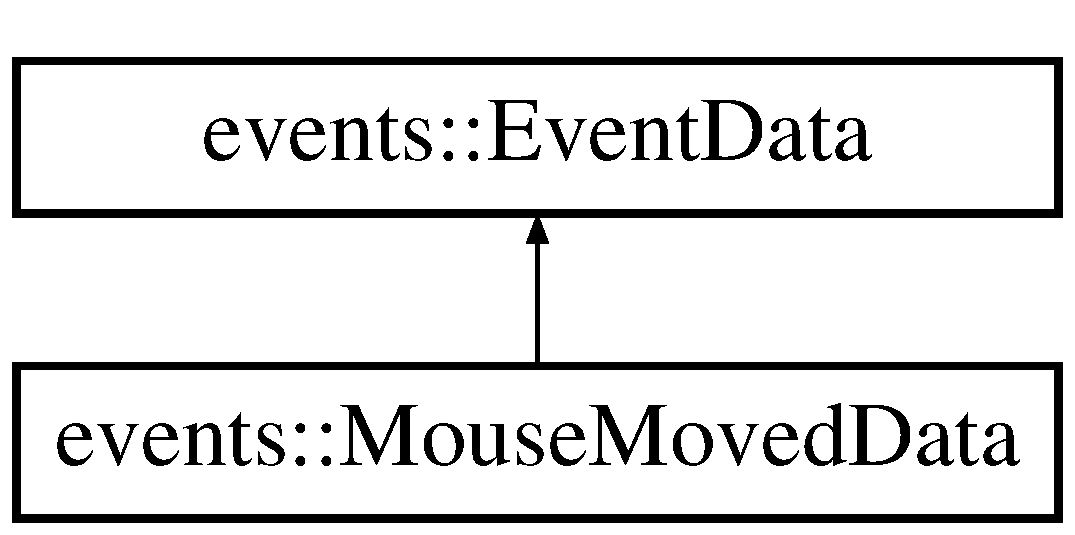
\includegraphics[height=2.000000cm]{structevents_1_1_mouse_moved_data}
\end{center}
\end{figure}
\subsection*{Public Attributes}
\begin{DoxyCompactItemize}
\item 
\hypertarget{structevents_1_1_mouse_moved_data_ad94258e6205be851ad91d5722a63f4c7}{}glm\+::ivec2 {\bfseries mouse\+Position}\label{structevents_1_1_mouse_moved_data_ad94258e6205be851ad91d5722a63f4c7}

\end{DoxyCompactItemize}


The documentation for this struct was generated from the following file\+:\begin{DoxyCompactItemize}
\item 
C\+:/\+Users/\+Simon/\+Documents/\+Visual Studio 2013/\+Projects/\+Ace\+Engine/\+Source/\+Ace\+Engine/Event\+Data.\+h\end{DoxyCompactItemize}

\hypertarget{struct_music_component}{}\section{Music\+Component Struct Reference}
\label{struct_music_component}\index{Music\+Component@{Music\+Component}}
\subsection*{Public Attributes}
\begin{DoxyCompactItemize}
\item 
\hypertarget{struct_music_component_ac6de34253b1d596cb4182b6f2e889123}{}std\+::string {\bfseries file\+Path}\label{struct_music_component_ac6de34253b1d596cb4182b6f2e889123}

\item 
\hypertarget{struct_music_component_a2d77aeaa1b223d31b66f5dc2c5664b19}{}Entity\+Id {\bfseries entity\+Id}\label{struct_music_component_a2d77aeaa1b223d31b66f5dc2c5664b19}

\item 
\hypertarget{struct_music_component_a6b028c0482d92185166d4bf4831bdf65}{}Element\+Id {\bfseries component\+Id}\label{struct_music_component_a6b028c0482d92185166d4bf4831bdf65}

\item 
\hypertarget{struct_music_component_aedb6b53bff9de828367c32cfeffbeab0}{}bool {\bfseries is\+Playing} = false\label{struct_music_component_aedb6b53bff9de828367c32cfeffbeab0}

\item 
\hypertarget{struct_music_component_a9800e5338cb7ebfbb60e40bb346c6823}{}bool {\bfseries is\+Looping} = true\label{struct_music_component_a9800e5338cb7ebfbb60e40bb346c6823}

\end{DoxyCompactItemize}


The documentation for this struct was generated from the following file\+:\begin{DoxyCompactItemize}
\item 
C\+:/\+Users/\+Simon/\+Documents/\+Visual Studio 2013/\+Projects/\+Ace\+Engine/\+Source/\+Ace\+Engine/Music\+Component.\+h\end{DoxyCompactItemize}

\hypertarget{class_packed_array}{}\section{Packed\+Array$<$ T $>$ Class Template Reference}
\label{class_packed_array}\index{Packed\+Array$<$ T $>$@{Packed\+Array$<$ T $>$}}
\subsection*{Classes}
\begin{DoxyCompactItemize}
\item 
class \hyperlink{class_packed_array_1_1_const_iterator}{Const\+Iterator}
\item 
class \hyperlink{class_packed_array_1_1_iterator}{Iterator}
\end{DoxyCompactItemize}
\subsection*{Public Member Functions}
\begin{DoxyCompactItemize}
\item 
\hypertarget{class_packed_array_a717fdda304b2c1f1e5c0d73c9d596699}{}{\bfseries Packed\+Array} (size\+\_\+t element\+Count)\label{class_packed_array_a717fdda304b2c1f1e5c0d73c9d596699}

\item 
\hypertarget{class_packed_array_a186f80f552a63554810ace6ee70e7e07}{}Element\+Id {\bfseries add} ()\label{class_packed_array_a186f80f552a63554810ace6ee70e7e07}

\item 
\hypertarget{class_packed_array_a74de2ef74ee2e8529b8d1a585e2b2331}{}void {\bfseries remove} (Element\+Id id)\label{class_packed_array_a74de2ef74ee2e8529b8d1a585e2b2331}

\item 
\hypertarget{class_packed_array_a2028e1a60f64ea46a821dd6093e92127}{}T $\ast$ {\bfseries lookup} (Element\+Id id)\label{class_packed_array_a2028e1a60f64ea46a821dd6093e92127}

\item 
\hypertarget{class_packed_array_af26675ecb16de2bafcc1e2e453235772}{}void {\bfseries iterate\+Function} (std\+::function$<$ void(T $\ast$)$>$ it\+Function)\label{class_packed_array_af26675ecb16de2bafcc1e2e453235772}

\item 
\hypertarget{class_packed_array_ad4f4b041ee820b5913ae9cd2805b5b24}{}T $\ast$ {\bfseries get\+Element\+Array} ()\label{class_packed_array_ad4f4b041ee820b5913ae9cd2805b5b24}

\item 
\hypertarget{class_packed_array_ae553569818eddf37f9268d45611ebee9}{}const T $\ast$ {\bfseries get\+Element\+Array} () const \label{class_packed_array_ae553569818eddf37f9268d45611ebee9}

\item 
\hypertarget{class_packed_array_a27fbfb13af910af1c2bc0c640def2070}{}unsigned int {\bfseries length} () const \label{class_packed_array_a27fbfb13af910af1c2bc0c640def2070}

\item 
\hypertarget{class_packed_array_a1aa30eddbe633324a94d84768ec86c84}{}\hyperlink{class_packed_array_1_1_iterator}{Iterator} {\bfseries begin} ()\label{class_packed_array_a1aa30eddbe633324a94d84768ec86c84}

\item 
\hypertarget{class_packed_array_af97fc05be0f100f5176743598b0bf8a2}{}\hyperlink{class_packed_array_1_1_iterator}{Iterator} {\bfseries end} ()\label{class_packed_array_af97fc05be0f100f5176743598b0bf8a2}

\item 
\hypertarget{class_packed_array_a674e7cc28a8aada5ba86c46fa3f436a6}{}\hyperlink{class_packed_array_1_1_const_iterator}{Const\+Iterator} {\bfseries begin} () const \label{class_packed_array_a674e7cc28a8aada5ba86c46fa3f436a6}

\item 
\hypertarget{class_packed_array_ab6e68fd1151b8281a0a639a6561a61ab}{}\hyperlink{class_packed_array_1_1_const_iterator}{Const\+Iterator} {\bfseries end} () const \label{class_packed_array_ab6e68fd1151b8281a0a639a6561a61ab}

\end{DoxyCompactItemize}


The documentation for this class was generated from the following file\+:\begin{DoxyCompactItemize}
\item 
C\+:/\+Users/\+Simon/\+Documents/\+Visual Studio 2013/\+Projects/\+Ace\+Engine/\+Source/\+Ace\+Engine/Packed\+Array.\+h\end{DoxyCompactItemize}

\hypertarget{class_physics_system}{}\section{Physics\+System Class Reference}
\label{class_physics_system}\index{Physics\+System@{Physics\+System}}
\subsection*{Public Member Functions}
\begin{DoxyCompactItemize}
\item 
\hypertarget{class_physics_system_af0e1507b77930b4a837ae64f654c502c}{}{\bfseries Physics\+System} (\hyperlink{class_entity_world}{Entity\+World} $\ast$entity\+World)\label{class_physics_system_af0e1507b77930b4a837ae64f654c502c}

\item 
\hypertarget{class_physics_system_a82f2b0b10a8b4c736fe4504678bbde23}{}void {\bfseries start} ()\label{class_physics_system_a82f2b0b10a8b4c736fe4504678bbde23}

\item 
\hypertarget{class_physics_system_a7e97af2ff3ac8bf879ab289397eb939c}{}void {\bfseries update} (float delta\+Time)\label{class_physics_system_a7e97af2ff3ac8bf879ab289397eb939c}

\end{DoxyCompactItemize}


The documentation for this class was generated from the following files\+:\begin{DoxyCompactItemize}
\item 
C\+:/\+Users/\+Simon/\+Documents/\+Visual Studio 2013/\+Projects/\+Ace\+Engine/\+Source/\+Ace\+Engine/Physics\+System.\+h\item 
C\+:/\+Users/\+Simon/\+Documents/\+Visual Studio 2013/\+Projects/\+Ace\+Engine/\+Source/\+Ace\+Engine/Physics\+System.\+cpp\end{DoxyCompactItemize}

\hypertarget{struct_player_component}{}\section{Player\+Component Struct Reference}
\label{struct_player_component}\index{Player\+Component@{Player\+Component}}
\subsection*{Public Attributes}
\begin{DoxyCompactItemize}
\item 
\hypertarget{struct_player_component_aa0575c3282d6efc66f1bf0fdbf16ced1}{}Entity\+Id {\bfseries entity\+Id}\label{struct_player_component_aa0575c3282d6efc66f1bf0fdbf16ced1}

\item 
\hypertarget{struct_player_component_a78ce9ae88dba1fb44048564dbd26c519}{}Element\+Id {\bfseries component\+Id}\label{struct_player_component_a78ce9ae88dba1fb44048564dbd26c519}

\end{DoxyCompactItemize}


The documentation for this struct was generated from the following file\+:\begin{DoxyCompactItemize}
\item 
C\+:/\+Users/\+Simon/\+Documents/\+Visual Studio 2013/\+Projects/\+Ace\+Engine/\+Source/\+Ace\+Engine/Player\+Component.\+h\end{DoxyCompactItemize}

\hypertarget{structevents_1_1_play_sound_data}{}\section{events\+:\+:Play\+Sound\+Data Struct Reference}
\label{structevents_1_1_play_sound_data}\index{events\+::\+Play\+Sound\+Data@{events\+::\+Play\+Sound\+Data}}
Inheritance diagram for events\+:\+:Play\+Sound\+Data\+:\begin{figure}[H]
\begin{center}
\leavevmode
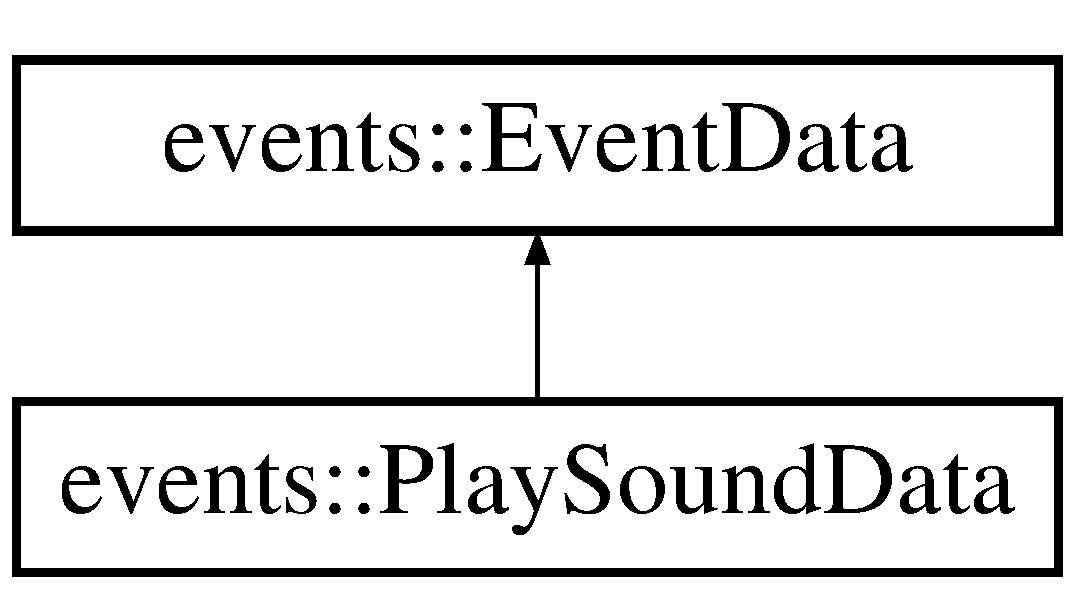
\includegraphics[height=2.000000cm]{structevents_1_1_play_sound_data}
\end{center}
\end{figure}
\subsection*{Public Attributes}
\begin{DoxyCompactItemize}
\item 
\hypertarget{structevents_1_1_play_sound_data_a3d40888a5a2d96d97e276148289ff49e}{}std\+::string {\bfseries path}\label{structevents_1_1_play_sound_data_a3d40888a5a2d96d97e276148289ff49e}

\end{DoxyCompactItemize}


The documentation for this struct was generated from the following file\+:\begin{DoxyCompactItemize}
\item 
C\+:/\+Users/\+Simon/\+Documents/\+Visual Studio 2013/\+Projects/\+Ace\+Engine/\+Source/\+Ace\+Engine/Event\+Data.\+h\end{DoxyCompactItemize}

\hypertarget{class_render_system}{}\section{Render\+System Class Reference}
\label{class_render_system}\index{Render\+System@{Render\+System}}
\subsection*{Public Member Functions}
\begin{DoxyCompactItemize}
\item 
\hypertarget{class_render_system_af65036a0ffb0814f91ae3aea428de1ec}{}{\bfseries Render\+System} (\hyperlink{class_entity_world}{Entity\+World} $\ast$entity\+World, \hyperlink{class_resource_loader}{Resource\+Loader}$<$ \hyperlink{struct_texture}{Texture} $>$ $\ast$texture\+Loader, \hyperlink{class_resource_loader}{Resource\+Loader}$<$ \hyperlink{struct_shader}{Shader} $>$ $\ast$shader\+Loader)\label{class_render_system_af65036a0ffb0814f91ae3aea428de1ec}

\item 
\hypertarget{class_render_system_adb1c97f7b6e3b4f85a7f0fd4d71e9bb5}{}void {\bfseries start} (unsigned int screen\+Size\+X, unsigned int screen\+Size\+Y)\label{class_render_system_adb1c97f7b6e3b4f85a7f0fd4d71e9bb5}

\item 
\hypertarget{class_render_system_aced51713f94b6f51ecf08d0520af1578}{}void {\bfseries update} (float delta\+Time, bool \&running)\label{class_render_system_aced51713f94b6f51ecf08d0520af1578}

\end{DoxyCompactItemize}


The documentation for this class was generated from the following files\+:\begin{DoxyCompactItemize}
\item 
C\+:/\+Users/\+Simon/\+Documents/\+Visual Studio 2013/\+Projects/\+Ace\+Engine/\+Source/\+Ace\+Engine/Render\+System.\+h\item 
C\+:/\+Users/\+Simon/\+Documents/\+Visual Studio 2013/\+Projects/\+Ace\+Engine/\+Source/\+Ace\+Engine/Render\+System.\+cpp\end{DoxyCompactItemize}

\hypertarget{class_resource_loader}{}\section{Resource\+Loader$<$ T $>$ Class Template Reference}
\label{class_resource_loader}\index{Resource\+Loader$<$ T $>$@{Resource\+Loader$<$ T $>$}}
\subsection*{Public Member Functions}
\begin{DoxyCompactItemize}
\item 
\hypertarget{class_resource_loader_accf0b5f190bc90853aa94e5037bdf9fc}{}std\+::vector$<$ T $\ast$ $>$ \& {\bfseries get\+Unitialized\+Resources} ()\label{class_resource_loader_accf0b5f190bc90853aa94e5037bdf9fc}

\item 
\hypertarget{class_resource_loader_ad2eb3670def91713850979611dc9e1c6}{}std\+::unordered\+\_\+map$<$ std\+::string, T $>$ \& {\bfseries get\+Resources} ()\label{class_resource_loader_ad2eb3670def91713850979611dc9e1c6}

\item 
\hypertarget{class_resource_loader_af24b628b1ce7a778098de29506f377bf}{}T $\ast$ {\bfseries load} (std\+::string resource\+Path)\label{class_resource_loader_af24b628b1ce7a778098de29506f377bf}

\end{DoxyCompactItemize}


The documentation for this class was generated from the following files\+:\begin{DoxyCompactItemize}
\item 
C\+:/\+Users/\+Simon/\+Documents/\+Visual Studio 2013/\+Projects/\+Ace\+Engine/\+Source/\+Ace\+Engine/Component\+Serializer.\+h\item 
C\+:/\+Users/\+Simon/\+Documents/\+Visual Studio 2013/\+Projects/\+Ace\+Engine/\+Source/\+Ace\+Engine/Resource\+Loader.\+h\end{DoxyCompactItemize}

\hypertarget{struct_rigidbody_component}{}\section{Rigidbody\+Component Struct Reference}
\label{struct_rigidbody_component}\index{Rigidbody\+Component@{Rigidbody\+Component}}
\subsection*{Public Attributes}
\begin{DoxyCompactItemize}
\item 
\hypertarget{struct_rigidbody_component_a6184693037f60b0211a79af3e2a4f665}{}Entity\+Id {\bfseries entity\+Id}\label{struct_rigidbody_component_a6184693037f60b0211a79af3e2a4f665}

\item 
\hypertarget{struct_rigidbody_component_ae388fa1df4240329076321adcd7cbc70}{}Element\+Id {\bfseries component\+Id}\label{struct_rigidbody_component_ae388fa1df4240329076321adcd7cbc70}

\item 
\hypertarget{struct_rigidbody_component_ad3f18bbe51bd85b3bf805ca9aee1ab9a}{}physx\+::\+Px\+Rigid\+Dynamic $\ast$ {\bfseries rigidbody} = nullptr\label{struct_rigidbody_component_ad3f18bbe51bd85b3bf805ca9aee1ab9a}

\end{DoxyCompactItemize}


The documentation for this struct was generated from the following file\+:\begin{DoxyCompactItemize}
\item 
C\+:/\+Users/\+Simon/\+Documents/\+Visual Studio 2013/\+Projects/\+Ace\+Engine/\+Source/\+Ace\+Engine/Rigidbody\+Component.\+h\end{DoxyCompactItemize}

\hypertarget{class_scene_importer}{}\section{Scene\+Importer Class Reference}
\label{class_scene_importer}\index{Scene\+Importer@{Scene\+Importer}}
\subsection*{Public Member Functions}
\begin{DoxyCompactItemize}
\item 
\hypertarget{class_scene_importer_a4ea30b104fd5b6532bb9b803288e53b7}{}{\bfseries Scene\+Importer} (\hyperlink{class_entity_world}{Entity\+World} $\ast$entity\+World, \hyperlink{class_resource_loader}{Resource\+Loader}$<$ \hyperlink{struct_texture}{Texture} $>$ $\ast$texture\+Loader, \hyperlink{class_resource_loader}{Resource\+Loader}$<$ \hyperlink{struct_shader}{Shader} $>$ $\ast$shader\+Loader)\label{class_scene_importer_a4ea30b104fd5b6532bb9b803288e53b7}

\item 
\hypertarget{class_scene_importer_a0079dcab3cda85d2a0b0176563a0032b}{}void {\bfseries load\+Scene} (unsigned int entity\+Id, const char $\ast$scene\+Path, std\+::string shader)\label{class_scene_importer_a0079dcab3cda85d2a0b0176563a0032b}

\end{DoxyCompactItemize}


The documentation for this class was generated from the following files\+:\begin{DoxyCompactItemize}
\item 
C\+:/\+Users/\+Simon/\+Documents/\+Visual Studio 2013/\+Projects/\+Ace\+Engine/\+Source/\+Ace\+Engine/Scene\+Importer.\+h\item 
C\+:/\+Users/\+Simon/\+Documents/\+Visual Studio 2013/\+Projects/\+Ace\+Engine/\+Source/\+Ace\+Engine/Scene\+Importer.\+cpp\end{DoxyCompactItemize}

\hypertarget{class_scene_loader}{}\section{Scene\+Loader Class Reference}
\label{class_scene_loader}\index{Scene\+Loader@{Scene\+Loader}}
\subsection*{Public Member Functions}
\begin{DoxyCompactItemize}
\item 
\hypertarget{class_scene_loader_a067bebc3d013526109b60e2c90906ab3}{}{\bfseries Scene\+Loader} (\hyperlink{class_entity_world}{Entity\+World} $\ast$entity\+World, \hyperlink{class_resource_loader}{Resource\+Loader}$<$ \hyperlink{struct_texture}{Texture} $>$ $\ast$texture\+Loader, \hyperlink{class_resource_loader}{Resource\+Loader}$<$ \hyperlink{struct_shader}{Shader} $>$ $\ast$shader\+Loader)\label{class_scene_loader_a067bebc3d013526109b60e2c90906ab3}

\item 
\hypertarget{class_scene_loader_ae5d06398432cf57635e6bdff4e61376d}{}bool {\bfseries load\+Scene} (const std\+::string \&file\+Path)\label{class_scene_loader_ae5d06398432cf57635e6bdff4e61376d}

\end{DoxyCompactItemize}


The documentation for this class was generated from the following files\+:\begin{DoxyCompactItemize}
\item 
C\+:/\+Users/\+Simon/\+Documents/\+Visual Studio 2013/\+Projects/\+Ace\+Engine/\+Source/\+Ace\+Engine/Scene\+Loader.\+h\item 
C\+:/\+Users/\+Simon/\+Documents/\+Visual Studio 2013/\+Projects/\+Ace\+Engine/\+Source/\+Ace\+Engine/Scene\+Loader.\+cpp\end{DoxyCompactItemize}

\hypertarget{struct_shader}{}\section{Shader Struct Reference}
\label{struct_shader}\index{Shader@{Shader}}
\subsection*{Public Attributes}
\begin{DoxyCompactItemize}
\item 
\hypertarget{struct_shader_a5c62b75f7315004d5584df5ca9f8b7b6}{}std\+::map$<$ const char $\ast$, unsigned int $>$ {\bfseries uniform\+Locations}\label{struct_shader_a5c62b75f7315004d5584df5ca9f8b7b6}

\item 
\hypertarget{struct_shader_a85a5911a2984cfd52ca4ed72ebd1e3c8}{}std\+::map$<$ const char $\ast$, unsigned int $>$ {\bfseries uniform\+Block\+Indices}\label{struct_shader_a85a5911a2984cfd52ca4ed72ebd1e3c8}

\item 
\hypertarget{struct_shader_a1e49a403b16a5b27e6f203cdf41c6e5f}{}std\+::string {\bfseries path}\label{struct_shader_a1e49a403b16a5b27e6f203cdf41c6e5f}

\item 
\hypertarget{struct_shader_af3eee7628d291077cfa66dcc83df83a2}{}unsigned int {\bfseries id}\label{struct_shader_af3eee7628d291077cfa66dcc83df83a2}

\item 
\hypertarget{struct_shader_a354f7d1afcd38ab33c3f689ba968d4f3}{}unsigned int {\bfseries vertex\+Shader}\label{struct_shader_a354f7d1afcd38ab33c3f689ba968d4f3}

\item 
\hypertarget{struct_shader_a344fb10044edfde57cbd6edf267832a9}{}unsigned int {\bfseries fragment\+Shader}\label{struct_shader_a344fb10044edfde57cbd6edf267832a9}

\end{DoxyCompactItemize}


The documentation for this struct was generated from the following file\+:\begin{DoxyCompactItemize}
\item 
C\+:/\+Users/\+Simon/\+Documents/\+Visual Studio 2013/\+Projects/\+Ace\+Engine/\+Source/\+Ace\+Engine/Shader.\+h\end{DoxyCompactItemize}

\hypertarget{struct_skybox_component}{}\section{Skybox\+Component Struct Reference}
\label{struct_skybox_component}\index{Skybox\+Component@{Skybox\+Component}}
\subsection*{Public Attributes}
\begin{DoxyCompactItemize}
\item 
\hypertarget{struct_skybox_component_a2f9e5017d59c212447a9270e2ddd4aa0}{}\hyperlink{struct_texture}{Texture} $\ast$ {\bfseries textures} \mbox{[}6\mbox{]}\label{struct_skybox_component_a2f9e5017d59c212447a9270e2ddd4aa0}

\item 
\hypertarget{struct_skybox_component_a04337bb57901881bc389a18e941b261d}{}Entity\+Id {\bfseries entity\+Id}\label{struct_skybox_component_a04337bb57901881bc389a18e941b261d}

\item 
\hypertarget{struct_skybox_component_abc4e5c051cec14bfefbb63fb3f5724c2}{}Element\+Id {\bfseries component\+Id}\label{struct_skybox_component_abc4e5c051cec14bfefbb63fb3f5724c2}

\item 
\hypertarget{struct_skybox_component_a794e5aa378c97d2bd5b276a7b048156c}{}unsigned int {\bfseries cubemap\+Id}\label{struct_skybox_component_a794e5aa378c97d2bd5b276a7b048156c}

\end{DoxyCompactItemize}


The documentation for this struct was generated from the following file\+:\begin{DoxyCompactItemize}
\item 
C\+:/\+Users/\+Simon/\+Documents/\+Visual Studio 2013/\+Projects/\+Ace\+Engine/\+Source/\+Ace\+Engine/Skybox\+Component.\+h\end{DoxyCompactItemize}

\hypertarget{struct_sound}{}\section{Sound Struct Reference}
\label{struct_sound}\index{Sound@{Sound}}
\subsection*{Public Attributes}
\begin{DoxyCompactItemize}
\item 
\hypertarget{struct_sound_a98783abfbc6344ce4160228714e53232}{}sf\+::\+Sound\+Buffer {\bfseries buffer}\label{struct_sound_a98783abfbc6344ce4160228714e53232}

\item 
\hypertarget{struct_sound_a87fb9425d23babf50354d587f4fc0417}{}std\+::string {\bfseries path}\label{struct_sound_a87fb9425d23babf50354d587f4fc0417}

\item 
\hypertarget{struct_sound_aa72b89f2aa57aa33794e7d6653a7f993}{}bool {\bfseries is\+Loaded} = false\label{struct_sound_aa72b89f2aa57aa33794e7d6653a7f993}

\end{DoxyCompactItemize}


The documentation for this struct was generated from the following file\+:\begin{DoxyCompactItemize}
\item 
C\+:/\+Users/\+Simon/\+Documents/\+Visual Studio 2013/\+Projects/\+Ace\+Engine/\+Source/\+Ace\+Engine/Sound.\+h\end{DoxyCompactItemize}

\hypertarget{struct_terrain_component}{}\section{Terrain\+Component Struct Reference}
\label{struct_terrain_component}\index{Terrain\+Component@{Terrain\+Component}}
\subsection*{Public Attributes}
\begin{DoxyCompactItemize}
\item 
\hypertarget{struct_terrain_component_a2a0f475fefcd59a27ba8364d397d0290}{}std\+::vector$<$ \hyperlink{struct_terrain_vertex_data}{Terrain\+Vertex\+Data} $>$ {\bfseries terrain\+Data}\label{struct_terrain_component_a2a0f475fefcd59a27ba8364d397d0290}

\item 
\hypertarget{struct_terrain_component_acfd3001b31459d14944f9c00f4a96786}{}std\+::vector$<$ unsigned int $>$ {\bfseries terrain\+Indices}\label{struct_terrain_component_acfd3001b31459d14944f9c00f4a96786}

\item 
\hypertarget{struct_terrain_component_acd777157fcd33430b38d7a1c71bdc338}{}\hyperlink{struct_texture}{Texture} $\ast$ {\bfseries height\+Texture} = nullptr\label{struct_terrain_component_acd777157fcd33430b38d7a1c71bdc338}

\item 
\hypertarget{struct_terrain_component_af4b0860f724b66135813dba761d0bf97}{}\hyperlink{struct_material}{Material} $\ast$ {\bfseries material}\label{struct_terrain_component_af4b0860f724b66135813dba761d0bf97}

\item 
\hypertarget{struct_terrain_component_a2cdc200c35bb00265f21db10a9df4470}{}bt\+Collision\+Shape $\ast$ {\bfseries collision\+Shape} = nullptr\label{struct_terrain_component_a2cdc200c35bb00265f21db10a9df4470}

\item 
\hypertarget{struct_terrain_component_a4ffee7106d10b44c6025ca2dcc3c9ae8}{}Entity\+Id {\bfseries entity\+Id}\label{struct_terrain_component_a4ffee7106d10b44c6025ca2dcc3c9ae8}

\item 
\hypertarget{struct_terrain_component_a377ad2a5de993981a686b9251e95b290}{}Element\+Id {\bfseries component\+Id}\label{struct_terrain_component_a377ad2a5de993981a686b9251e95b290}

\item 
\hypertarget{struct_terrain_component_a3c5ef92da76bd61b3c9a70ac04f500e4}{}unsigned int {\bfseries vao}\label{struct_terrain_component_a3c5ef92da76bd61b3c9a70ac04f500e4}

\item 
\hypertarget{struct_terrain_component_a5ef9db788f2491af739c7d6b451db71e}{}unsigned int {\bfseries vbo}\label{struct_terrain_component_a5ef9db788f2491af739c7d6b451db71e}

\item 
\hypertarget{struct_terrain_component_aafbf4c13f411fcf31cdfdef44d88c199}{}unsigned int {\bfseries ibo}\label{struct_terrain_component_aafbf4c13f411fcf31cdfdef44d88c199}

\item 
\hypertarget{struct_terrain_component_a0ce843ffedafa48c4985ffa592a6b652}{}unsigned int {\bfseries indices\+Num} = 0\label{struct_terrain_component_a0ce843ffedafa48c4985ffa592a6b652}

\item 
\hypertarget{struct_terrain_component_a4fce750323d620ffb602f69815857cd6}{}unsigned int {\bfseries tiling} = 20\label{struct_terrain_component_a4fce750323d620ffb602f69815857cd6}

\item 
\hypertarget{struct_terrain_component_a8dbb4d6cfaa23cd174b12ff614505512}{}float {\bfseries max\+Height} = 155.\+0f\label{struct_terrain_component_a8dbb4d6cfaa23cd174b12ff614505512}

\item 
\hypertarget{struct_terrain_component_a3c382157822187a652730d2841a21412}{}float {\bfseries terrain\+Scale} = 1.\+0f\label{struct_terrain_component_a3c382157822187a652730d2841a21412}

\end{DoxyCompactItemize}


The documentation for this struct was generated from the following file\+:\begin{DoxyCompactItemize}
\item 
C\+:/\+Users/\+Simon/\+Documents/\+Visual Studio 2013/\+Projects/\+Ace\+Engine/\+Source/\+Ace\+Engine/Terrain\+Component.\+h\end{DoxyCompactItemize}

\hypertarget{class_terrain_system}{}\section{Terrain\+System Class Reference}
\label{class_terrain_system}\index{Terrain\+System@{Terrain\+System}}
\subsection*{Public Member Functions}
\begin{DoxyCompactItemize}
\item 
\hypertarget{class_terrain_system_a8e1cde2ee844c9f7ab890d65f07d5798}{}{\bfseries Terrain\+System} (\hyperlink{class_entity_world}{Entity\+World} $\ast$entity\+World)\label{class_terrain_system_a8e1cde2ee844c9f7ab890d65f07d5798}

\item 
\hypertarget{class_terrain_system_a27419922782976d8edcc759272344c21}{}void {\bfseries start} ()\label{class_terrain_system_a27419922782976d8edcc759272344c21}

\end{DoxyCompactItemize}


The documentation for this class was generated from the following files\+:\begin{DoxyCompactItemize}
\item 
C\+:/\+Users/\+Simon/\+Documents/\+Visual Studio 2013/\+Projects/\+Ace\+Engine/\+Source/\+Ace\+Engine/Terrain\+System.\+h\item 
C\+:/\+Users/\+Simon/\+Documents/\+Visual Studio 2013/\+Projects/\+Ace\+Engine/\+Source/\+Ace\+Engine/Terrain\+System.\+cpp\end{DoxyCompactItemize}

\hypertarget{struct_terrain_vertex_data}{}\section{Terrain\+Vertex\+Data Struct Reference}
\label{struct_terrain_vertex_data}\index{Terrain\+Vertex\+Data@{Terrain\+Vertex\+Data}}
\subsection*{Public Attributes}
\begin{DoxyCompactItemize}
\item 
\hypertarget{struct_terrain_vertex_data_ae6bef080a5485a5948375d42fe701475}{}glm\+::vec2 {\bfseries position}\label{struct_terrain_vertex_data_ae6bef080a5485a5948375d42fe701475}

\item 
\hypertarget{struct_terrain_vertex_data_a1b63c97ef2e95771d2ab58bd12babf24}{}glm\+::vec3 {\bfseries normal}\label{struct_terrain_vertex_data_a1b63c97ef2e95771d2ab58bd12babf24}

\item 
\hypertarget{struct_terrain_vertex_data_a0a363e2014242dbeabacf52cc4cec5a2}{}glm\+::vec2 {\bfseries uv}\label{struct_terrain_vertex_data_a0a363e2014242dbeabacf52cc4cec5a2}

\end{DoxyCompactItemize}


The documentation for this struct was generated from the following file\+:\begin{DoxyCompactItemize}
\item 
C\+:/\+Users/\+Simon/\+Documents/\+Visual Studio 2013/\+Projects/\+Ace\+Engine/\+Source/\+Ace\+Engine/Terrain\+Component.\+h\end{DoxyCompactItemize}

\hypertarget{struct_texture}{}\section{Texture Struct Reference}
\label{struct_texture}\index{Texture@{Texture}}
\subsection*{Public Attributes}
\begin{DoxyCompactItemize}
\item 
\hypertarget{struct_texture_aca5a94887081662571f71c113a50da90}{}sf\+::\+Image {\bfseries image}\label{struct_texture_aca5a94887081662571f71c113a50da90}

\item 
\hypertarget{struct_texture_aa8ba4ade408b0df1fc9b6f605a4efd22}{}std\+::string {\bfseries path}\label{struct_texture_aa8ba4ade408b0df1fc9b6f605a4efd22}

\item 
\hypertarget{struct_texture_ab1c2077cdc453d9a42505975d1cd4daa}{}glm\+::uvec2 {\bfseries size}\label{struct_texture_ab1c2077cdc453d9a42505975d1cd4daa}

\item 
\hypertarget{struct_texture_aed42161a5c00b6020c85833401da6da6}{}unsigned int {\bfseries id}\label{struct_texture_aed42161a5c00b6020c85833401da6da6}

\item 
\hypertarget{struct_texture_ad83ed086abaa805a606a5ccd433f505c}{}Texture\+Type {\bfseries type} = Texture\+Type\+::\+Texture2\+D\label{struct_texture_ad83ed086abaa805a606a5ccd433f505c}

\item 
\hypertarget{struct_texture_a0f7ade2abc1ccc6611e9beba8e94c1d9}{}bool {\bfseries is\+Loaded} = false\label{struct_texture_a0f7ade2abc1ccc6611e9beba8e94c1d9}

\end{DoxyCompactItemize}


The documentation for this struct was generated from the following file\+:\begin{DoxyCompactItemize}
\item 
C\+:/\+Users/\+Simon/\+Documents/\+Visual Studio 2013/\+Projects/\+Ace\+Engine/\+Source/\+Ace\+Engine/Texture.\+h\end{DoxyCompactItemize}

\hypertarget{struct_transform_component}{}\section{Transform\+Component Struct Reference}
\label{struct_transform_component}\index{Transform\+Component@{Transform\+Component}}
\subsection*{Public Attributes}
\begin{DoxyCompactItemize}
\item 
\hypertarget{struct_transform_component_a92b2cb46b81ef72fd133885df47b0c77}{}Entity\+Id {\bfseries entity\+Id}\label{struct_transform_component_a92b2cb46b81ef72fd133885df47b0c77}

\item 
\hypertarget{struct_transform_component_a41210d33f1663aac14ad30ecc9951d87}{}Element\+Id {\bfseries component\+Id}\label{struct_transform_component_a41210d33f1663aac14ad30ecc9951d87}

\item 
\hypertarget{struct_transform_component_a07035d8d3a70e9935c2355ad0835e0d3}{}glm\+::vec3 {\bfseries position} = glm\+::vec3(0.\+0f)\label{struct_transform_component_a07035d8d3a70e9935c2355ad0835e0d3}

\item 
\hypertarget{struct_transform_component_a4655f45435c9b2403d54ebda6ffafc68}{}glm\+::vec3 {\bfseries scale} = glm\+::vec3(1.\+0f)\label{struct_transform_component_a4655f45435c9b2403d54ebda6ffafc68}

\item 
\hypertarget{struct_transform_component_ad7b9cc2ac98f6c0277e48ae6a1cc67dd}{}glm\+::quat {\bfseries rotation} = glm\+::quat()\label{struct_transform_component_ad7b9cc2ac98f6c0277e48ae6a1cc67dd}

\end{DoxyCompactItemize}


The documentation for this struct was generated from the following file\+:\begin{DoxyCompactItemize}
\item 
C\+:/\+Users/\+Simon/\+Documents/\+Visual Studio 2013/\+Projects/\+Ace\+Engine/\+Source/\+Ace\+Engine/Transform\+Component.\+h\end{DoxyCompactItemize}

\hypertarget{struct_vertex_data}{}\section{Vertex\+Data Struct Reference}
\label{struct_vertex_data}\index{Vertex\+Data@{Vertex\+Data}}
\subsection*{Public Attributes}
\begin{DoxyCompactItemize}
\item 
\hypertarget{struct_vertex_data_a2b9e13ce103a07c15e8769d7c2193702}{}glm\+::vec3 {\bfseries position}\label{struct_vertex_data_a2b9e13ce103a07c15e8769d7c2193702}

\item 
\hypertarget{struct_vertex_data_a62c7802a045b5cf3055bceead2472e41}{}glm\+::vec3 {\bfseries normal}\label{struct_vertex_data_a62c7802a045b5cf3055bceead2472e41}

\item 
\hypertarget{struct_vertex_data_a59d18bd0c51f802ad63a000d2521e9dc}{}glm\+::vec3 {\bfseries tangent}\label{struct_vertex_data_a59d18bd0c51f802ad63a000d2521e9dc}

\item 
\hypertarget{struct_vertex_data_adebd633d522750161e34c9659e2ed235}{}glm\+::vec3 {\bfseries bitangent}\label{struct_vertex_data_adebd633d522750161e34c9659e2ed235}

\item 
\hypertarget{struct_vertex_data_a7ff3d9f97b6a18665dcf3e43117eb1fb}{}glm\+::vec2 {\bfseries uv}\label{struct_vertex_data_a7ff3d9f97b6a18665dcf3e43117eb1fb}

\end{DoxyCompactItemize}


The documentation for this struct was generated from the following file\+:\begin{DoxyCompactItemize}
\item 
C\+:/\+Users/\+Simon/\+Documents/\+Visual Studio 2013/\+Projects/\+Ace\+Engine/\+Source/\+Ace\+Engine/Vertex\+Data.\+h\end{DoxyCompactItemize}

\hypertarget{structevents_1_1_window_created_data}{}\section{events\+:\+:Window\+Created\+Data Struct Reference}
\label{structevents_1_1_window_created_data}\index{events\+::\+Window\+Created\+Data@{events\+::\+Window\+Created\+Data}}
Inheritance diagram for events\+:\+:Window\+Created\+Data\+:\begin{figure}[H]
\begin{center}
\leavevmode
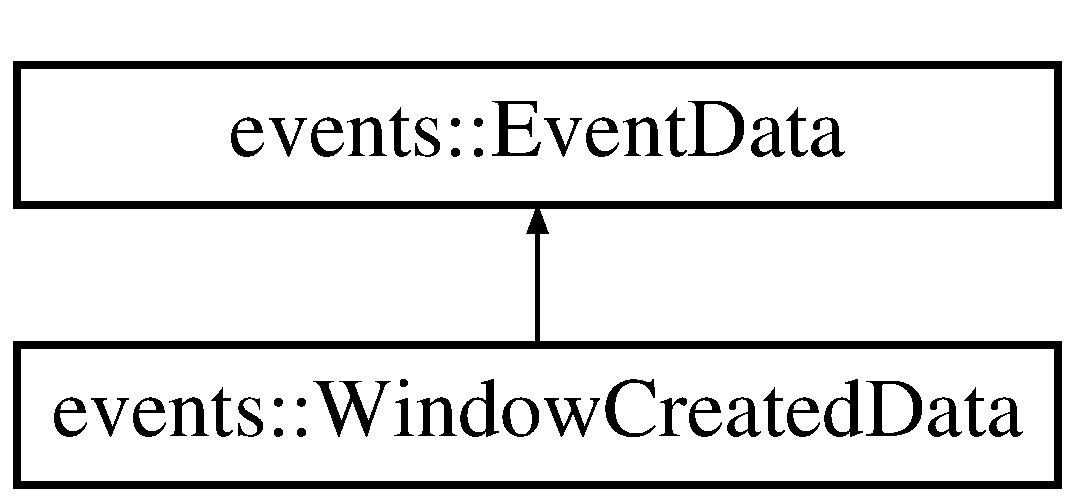
\includegraphics[height=2.000000cm]{structevents_1_1_window_created_data}
\end{center}
\end{figure}
\subsection*{Public Attributes}
\begin{DoxyCompactItemize}
\item 
\hypertarget{structevents_1_1_window_created_data_a4b28b3577391b16a811b013cfd5e75a8}{}sf\+::\+Window $\ast$ {\bfseries window}\label{structevents_1_1_window_created_data_a4b28b3577391b16a811b013cfd5e75a8}

\end{DoxyCompactItemize}


The documentation for this struct was generated from the following file\+:\begin{DoxyCompactItemize}
\item 
C\+:/\+Users/\+Simon/\+Documents/\+Visual Studio 2013/\+Projects/\+Ace\+Engine/\+Source/\+Ace\+Engine/Event\+Data.\+h\end{DoxyCompactItemize}

%--- End generated contents ---

% Index
\backmatter
\newpage
\phantomsection
\clearemptydoublepage
\addcontentsline{toc}{chapter}{Index}
\printindex

\end{document}
